\chapter{Standard Model and Supersymmetry}
\label{chap:SMSUSY}

This chapter presents an introduction to the \gls{sm} of particle physics, the theory that nowadays best describes the subatomic world. In Section \ref{sec:smsusy:sm} a general overview of the \gls{sm} is given. Section \ref{sec:smsusy:bsm} discusses the limitations of the SM, and some of the theoretical extensions proposed to overcome them. Finally Section \ref{sec:smsusy:susy} focuses on Supersymmetry, arguably one of the most promising of these extensions. Throughout this chapter (as well as in the rest of this thesis) we will use natural units; we will thus use energy units to describe masses, as the speed of light ($c$) and the Planck constant ($\hslash$) are set to unity.


\section{The Standard Model of Particle Physics}
\label{sec:smsusy:sm}

The \gls{sm} is a renormalizable gauge quantum field theory based on the group $SU(3) \times SU(2) \times U(1)$. It was developed in the second half of the 20th century \cite{Glashow:1961tr, Weinberg:1967tq, Salam:1980jd}, and since then the description that it gives of the elementary particles and of their interactions has been accurately tested by several experiments. Many experimental discoveries have been guided by the \gls{sm} predictions, including the discovery of the top quark \cite{Abachi:1994td, PhysRevLett.74.2626} and up to the latest one, the observation of the Higgs boson at the \gls{lhc} in July 2012 \cite{Aad:2012tfa, Chatrchyan:2012xdj}. 

\subsection{Particle content of the Standard Model}

In the \gls{sm}, particles are described as excitations of quantum fields. In the following paragraphs, we introduce the quantum field theory description of fermions and bosons.

\subsubsection*{Fermions}

Matter constituents are half-integer spin fields (fermions). Fermions are further divided into two categories based on the type of interaction they experience:
\begin{description}
\item[Leptons] which experience only the electroweak interaction.
\item[Quarks] which experience both the electroweak and the strong interaction.
\end{description}

Both leptons and quarks come in three generations, and conventionally the numbering of these generations follows an order of increasing mass. A summary of the \gls{sm} fermions is presented in Table \ref{tab:sm_fermions}. While it is possible to observe free leptons, quarks exist only in bound states (hadrons); this is because of the confinement property of the strong interaction, discussed in Section \ref{sec:strong}. Hadrons built of three quarks have spin $\frac{1}{2}$ and are named barions, while mesons are formed by two quarks and have integer spin.


The free Lagrangian of a fermion is given by:

\begin{equation}
 \mathcal{L}_{free} = \bar{\psi} \left( i \gamma^{\mu} \partial_{\mu} - m \right) \psi \, , \
 \label{eq:sm:dirac}
\end{equation}

\noindent where $\psi$ is the fermion field, $m$ its mass, $\gamma$ are the Dirac matrices and $\partial_{\mu}$ is the four-momentum derivative. 

\begin{table}[h]
\centering
\begin{tabular}{c|ccc|ccc}
\hline
 & \multicolumn{3}{c|}{Leptons} & \multicolumn{3}{c}{Quarks} \\
\hline
\hline
Generation & Flavor & Charge & Mass [GeV] & Flavor & Charge & Mass [GeV]\\
\hline
\hline
\multirow{2}*{$1^{st}$} & $\nu_e$ & 0   & $< 2 \times 10^{-9}$  & $u$ & +2/3 & $2.2 \times 10^{-3}$ \\
                        & $e$     & -1  & $5.1 \times 10^{-4}$ & $d$ & -1/3 & $4.8 \times 10^{-3}$ \\
\hline  
\multirow{2}*{$2^{nd}$} & $\nu_\mu$ & 0   & $< 2 \times 10^{-9}$  & $c$ & +2/3 & $ 1.27 $ \\
                        & $\mu$     & -1  & $ 0.10566  $ & $s$ & -1/3 & $ 0.096 $ \\
\hline                 
\multirow{2}*{$3^{rd}$} & $\nu_\tau$ & 0   & $< 2 \times 10^{-9}$  & $t$ & +2/3 & $ 173.2 $ \\
                        & $\tau$     & -1  & $ 1.77 $ & $b$ & -1/3 & $ 4.66 $ \\
\hline  
                 
%\multirow{2}*{Weak} & $W^{+}$, $W^{-}$    &  +1, -1 &  	$80.385$ $\pm0.015$ \\%  & $10^{-6}$\\
 
\end{tabular}
\caption[Standard Model Ferimons]{Fermion content of the Standard Model. Each particle is listed with its electric charge and mass \cite{Patrignani:2016xqp}.} 
\label{tab:sm_fermions}
\end{table}


\subsubsection*{Bosons}

Particles with integer spin are referred to as bosons. In the \gls{sm}, force carriers are described through spin-1 fields. 
The \gls{sm} includes also a spin-0 particle, the Higgs boson. Is the interaction with the Higgs boson field that allows all the other elementary particles to acquire mass, as described in Section \ref{sec:smsusy:ew}.

The Klein-Gordon Lagrangian governs the kinematics of spin-0 neutral particles:

\begin{equation}
\mathcal{L}_{\rm{free}} = \frac{1}{2} \partial^\mu \phi \partial_\mu \phi - \frac{1}{2} m^2 \phi ^2 ,
\end{equation}

 
\noindent while in the case of charged particles (described through a complex field) the Lagrangian becomes:

\begin{equation}
\mathcal{L}_{\rm{free}} =  \partial^\mu \phi \partial_\mu \phi^* -  m^2 \phi \phi^* .
\end{equation}


\noindent The two equations above describe scalar particles. In the case of a vector field $A^\mu$, the expression of the Lagrangian is the following: 

\begin{equation}
\mathcal{L}_{\rm{free}} =  - \frac{1}{4} F^{\mu \nu}F_{\mu \nu} +  \frac{1}{2} m^2 A^\mu A_\mu \, .
\label{eq:lproca}
\end{equation}

\noindent This is the Proca Lagrangian. In the case of a particle with zero mass, this reduces to the Maxwell Lagrangian:

\begin{equation}
\mathcal{L}_{free} =  - \frac{1}{4} F^{\mu \nu}F_{\mu \nu} ,
\label{eq:lmax}
\end{equation}


\noindent where $F^{\mu \nu} = \partial^\mu A_\nu - \partial^\nu A_\mu$.

\subsection{Interactions and gauge invariance}

The \gls{sm} describes all the interactions among elementary particles, except for gravity, for which nowadays no renormalizable quantum field theory is formulated. Table \ref{tab:sm_interazioni} presents a summary of the \gls{sm} interactions and the properties of the corresponding force carriers. More details about the strong and electroweak interactions are given in the following sections.

\begin{table}[h]
\centering
\begin{tabular}{llcc}
\hline
Interaction & Carrier & Electric Charge & Mass [GeV] \\% & $\alpha$ \\
\hline
\hline
Strong & Gluons (g)  & 0 & 0 \\ % & 10 \\
\hline
Electromagnetic & Photon ($\gamma$) & $< 10^{-27}$ & 0 \\%& $10^{-2}$ \\
\hline
\multirow{2}*{Weak} & $W^{+}$, $W^{-}$    &  +1, -1 &  	$80.385$  \\% $\pm0.015$  & $10^{-6}$\\
 & $Z$  & 0 &  	$91.1876$  \\% & $\pm0.0021$ \\
\hline
\end{tabular}
\caption[Interaction in the Standard Model]{Interaction in the Standard Model. Here the different force carriers are listed, with their electric charges and masses \cite{Patrignani:2016xqp}.} %; $\alpha$ is the coupling constant of the different interactions.}
\label{tab:sm_interazioni}
\end{table}


The interaction terms in the \gls{sm} Lagrangian are introduced by promoting an already existing global symmetry of the Lagrangian ($\theta$) to a local one ($\theta(x)$) function of the space-time coordinates. 
In general, given a Lagrangian globally invariant under a symmetry group, the fields transform as:
\begin{equation}
\psi \rightarrow e^{ig\theta^k \tau^k} \psi  \; ,
\end{equation}

\noindent where $g$ is the coupling constant of the filed $\psi$ under the interaction and $\tau^k$ are the generators of the group and obey commutation relations: 
\begin{equation}
\left[ \tau^i, \tau^j \right] = i f^{ijk} \tau^k \; . 
\end{equation}

\noindent In the equation above, $f^{ijk}$ is the structure constant of the group and is always zero for Abelian groups. Promoting this global  invariance to a local one ($\theta^k \rightarrow \theta^k(x)$) implies adding to the theory:
\begin{itemize}
\item A number of massless gauge fields $W_\mu^k$ equal to the number of generators of the symmetry group, that transform as 
\begin{equation}
W_\mu^k \rightarrow W_\mu^k + \partial_\mu \theta^k + g f^{klm} W_\mu^l \theta^m  \; .
\end{equation}
\item A covariant derivative: 
\begin{equation}
D_\mu = \partial_\mu - ig\tau^kW_\mu^k \; ,
\end{equation}

\noindent that substitutes the standard derivative in the Lagrangian.
\item A free Lagrangian for the vector fields as in Equation \ref{eq:lproca}, with:
\begin{equation}
F_{\mu \nu}^k = \partial_\mu W^k_\nu - \partial_\nu W^k_\mu + g f^{klm} W_\mu^l W_\nu^m \; .
\end{equation}
\noindent Note that the last term, of second order in the field, is present only for non-Abelian symmetry groups, since it is proportional to the structure constant. This has non-trivial consequences as the second-order term leads to self-interaction among the gauge fields.
\end{itemize}


The \gls{sm} is a theory invariant under $SU(3)_{C} \times SU(2)_{L} \times U(1)_{Y}$. Imposing local invariance under $SU(3)_{C}$ leads to the theory of strong interactions, while $SU(2)_{L} \times U(1)_{Y}$ is the symmetry whose breaking gives origin to the electroweak interactions. 

\subsection{Strong interaction}
\label{sec:strong}

\Gls{qcd} is the theory that describes strong interactions, based on the symmetry group $SU(3)_\mathrm{C}$, where the subscript C refers to the color, the quantum number associated with these interactions; this can assume three possible values denoted with red, blue and green. The observable states, hadrons, are color singlets, while quarks (anti-quarks) carry only one color (anti-color) charge. Since the symmetry group is non-Abelian, also the corresponding eight gauge bosons (gluons) carry a color charge (bi-color, with one color and one different anti-color) and therefore interact not only with quarks but also among themselves. Since $SU(3)_\mathrm{C}$ is believed to be an exact symmetry,  gluons are massless. 

The renormalization of a gauge theory leads to the definition of running coupling constants, whose value depend on the energy scale at which they are evaluated. In \gls{qcd}, at leading order the dependence of the coupling constant on the energy scale $Q$ is given by:

\begin{equation}
\alpha_\mathrm{s}(Q^2)=\frac{12\pi}{\left(11N_\mathrm{C}-2n_\mathrm{f}\right)\log{\frac{Q^2}{\Lambda_\mathrm{QCD}^2}}} \; , 
\label{eq:alfaQCD}
\end{equation}

\noindent where $N_\mathrm{C}$ is the number of colors, $n_\mathrm{f}$ is the number of quark flavors that are active (i.e. whose mass is lower than the energy scale) and $\Lambda_\mathrm{QCD}$ is the infrared cutoff scale that sets the limit of validity of the perturbative approximation. In \gls{qcd} $N_\mathrm{C} = 3$, so for $n_\mathrm{f}<16$ the coupling constant decreases with the increase of the energy scale of the process considered. This behavior has important consequences on the properties of the strong interaction:

\begin{itemize}
\item At high $Q^2$ (i.e. at small distances), $\alpha_\mathrm{s}$ becomes small enough for the perturbative approximation to be correct. In this case quarks and gluons behave as free particles; this behavior is referred to as asymptotic freedom \cite{PhysRevLett.30.1343, PhysRevLett.30.1346}.
\item When the momentum transfer is small (i.e. at large distances) $\alpha_\mathrm{s}$ is large; this gives rise to confinement: quarks can not be observed as isolated particles, as it is not possible to extract individual quarks from hadrons. When the distance between two quarks is increased, the potential energy increases as well, up to the point when it is energetically more favorable to create from the vacuum a quark-antiquark pair and thus a new hadron is formed.
\item In a collider experiment, quarks and gluons will create a collimated spray of hadrons, referred to as jet.
\end{itemize}

The evolution of the \gls{qcd} coupling constant with the energy scale has been verified experimentally, as shown in Figure \ref{fig:sm:alphas}.

\begin{figure}[ht]
\centering
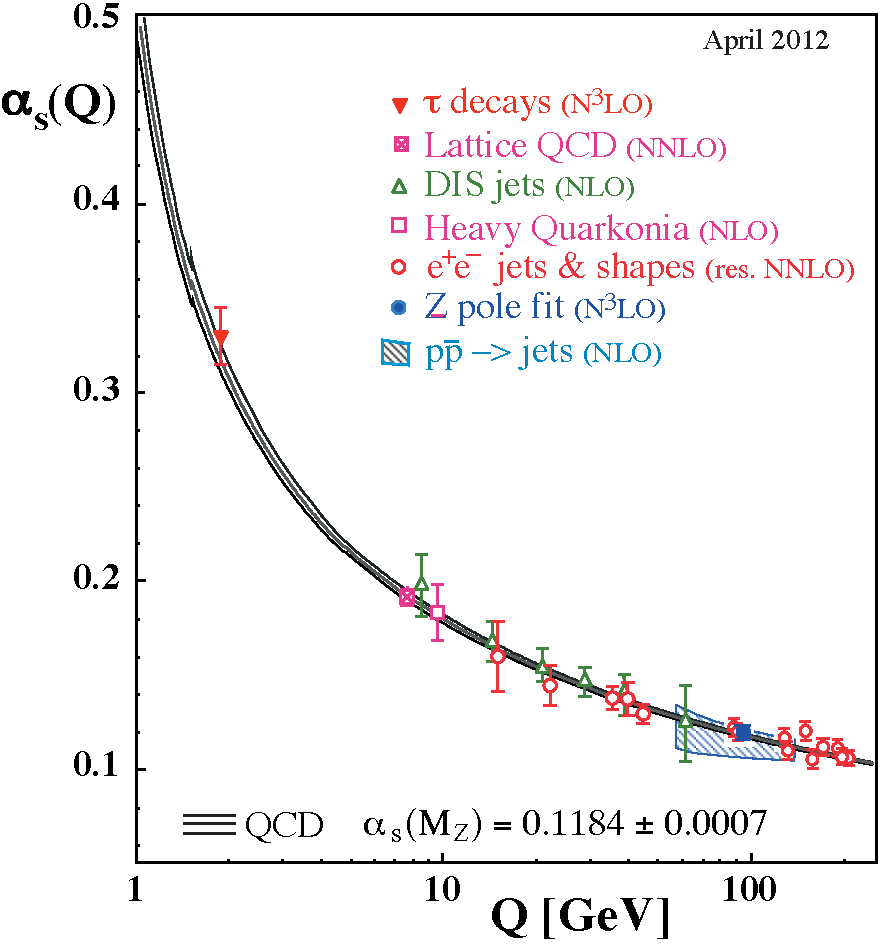
\includegraphics[width=0.5\textwidth]{figures/theory/asq-2011}
\caption{Evolution of the \gls{qcd} coupling constant $\alpha_\mathrm{s}$ with the energy scale. Figure from Ref \cite{Bethke:2012jm}.}
\label{fig:sm:alphas}
\end{figure}

\subsection{Electroweak interaction and Higgs-Englert-Brout mechanism}
\label{sec:smsusy:ew}

The theory of electroweak interactions is based on the symmetry group $SU(2)_\mathrm{L} \times U(1)_\mathrm{Y}$. This symmetry breaks at a scale around 100 GeV giving rise to the electromagnetic interaction, mediated by the photon, and to the weak interaction, mediated by the $Z$ and $W^{\pm}$ bosons  for neutral currents and charged currents respectively. The number of mediators, four, is the same as the number of generators of the symmetry group. 

The $SU(2)_\mathrm{L}$ part of the symmetry group governs the weak interactions, and the subscript L indicates that only left-handed particles participate to them. Left-handed and right-handed fields ($\psi_L$ and $\psi_R$ respectively) are defined through the chirality projectors $P_L$ and $P_R$:

\begin{equation}
\begin{aligned}
\psi_L = P_L \psi = \frac{(1 - \gamma_5)}{2} \psi, \\
\psi_R = P_R \psi = \frac{(1 + \gamma_5)}{2} \psi,
\end{aligned}
\label{eq:sm:LR}
\end{equation}

\noindent where $\gamma_5$ is defined as $\gamma_5 = i \gamma^0 \gamma^1 \gamma^2 \gamma^3 $. Looking back at Equation \ref{eq:sm:dirac}, it can be noted that, if we decompose the fermion field into its left-handed and right-handed components, the derivative term keeps $\psi_L$ and $\psi_R$ separated, while the mass term mixes them:
\begin{equation}
-m \bar \psi \psi = -m \bar \psi P_L^2 \psi - m \bar \psi P_R^2 \psi
	= -m \bar \psi_R \psi_L - m \bar \psi_L \psi_R \; .
\end{equation}


\noindent The covariant derivative for the  $SU(2)_\mathrm{L} \times U(1)_\mathrm{Y}$ group is:
\begin{equation}
\mathcal{D}_{\mu} = \partial_{\mu} - i g' B_\mu Y - ig W_\mu^k T^k \; ,
\label{eq:sm:covD}
\end{equation}

\noindent and substituting with this the regular derivative results in the interaction Lagrangian:
\begin{equation}
\mathcal{L}_{int}^{EW} = -\frac{g'}{2} \left( \bar{\psi} \gamma_\mu Y \psi \right) B^\mu - g \sum_k \left( \bar{\psi} \gamma_\mu T^k \psi  \right) W_k^\mu \; ,
\end{equation}

\noindent where we have introduced $T^k$, the weak isospin operator, and $Y$, the hypercharge operator (associated to the $U(1)_\mathrm{Y}$ group), and the respective coupling constants $g$ and $g'$. The quantum numbers of the $T^k$ and $Y$ operators relate to the electric charge $Q$ through the  Gell-Mann Nishijima relation:

\begin{equation}
Q = \frac{Y}{2} + T_3 \; ,
\label{eq:sm:Q}
\end{equation}

\noindent where $Y$ is the hypercharge quantum number and $T_3$ is the quantum number of the third component of the isospin. 

In the case of an $SU(2)$ symmetry, it is not possible to add directly to the Lagrangian a mass term for the vector bosons of the form in Equation \ref{eq:lproca}, as it would spoil the $SU(2)$ local invariance. The Higgs-Englert-Brout mechanism \cite{Englert:1964et, Higgs:1964pj, Higgs:1964ia} solves this problem through \gls{ssb} of the $SU(2)_\mathrm{L} \times U(1)_\mathrm{Y}$ invariance. The \gls{ssb} is obtained by adding to the theory one extra isospin doublet of complex scalar components, the Higgs field:

\begin{equation}
	\Phi = \left( \begin{array}{c} \phi^+  \\ \phi^0 \end{array} \right) \; .
\end{equation}
%	= \frac{1}{\sqrt{2}} \left( \begin{array}{c} \phi_1 + i \phi_2 \\ \phi_3 + i \phi_4 \end{array} \right)

\noindent This doublet has hypercharge $Y=1$ and isospin $T=\frac{1}{2}$; the first component has positive electric charge, while the second one is electrically neutral. The Lagrangian for this new field includes a kinetic and a potential term:

\begin{equation}
	\mathcal{L}_{\Phi} = ( \mathcal{D}_{\mu} \Phi)^{\dagger} (\mathcal{D}^{\mu} \Phi) - V(\Phi) \; ,
	\label{eq:LHiggs}
\end{equation}

\noindent where $\mathcal{D}_{\mu}$ is the covariant derivative defined in Equation \ref{eq:sm:covD} and the potential $V(\Phi)$ is given by:

\begin{equation}
 V(\Phi) =  \mu^2 \Phi^{\dagger} \Phi + \lambda (\Phi^{\dagger} \Phi)^2 \, . 
	\label{eq:hpot}
\end{equation}

\noindent The two real parameters $\mu^2$ and $\lambda$ relate respectively to the mass term and the strength of the self-interaction term. The shape of the potential depends on the value of these parameters:
\begin{itemize}
\item If $\lambda < 0$, the potential does not present any stable minima, and this case is therefore unphysical.
\item If $\lambda > 0$ and $\mu^2 > 0$ there is only one solution to the minimization of the potential, $\Phi=0$. This case is shown in Figure  \ref{fig:sm:HiggsV_1}.
\item If $\lambda > 0$ and $\mu^2 < 0$, the field acquires a \gls{vev} as the minima is not at zero; it lies instead on the points of the circumference such that:
\begin{equation}
\Phi^{\dagger} \Phi = \frac{\mu^2}{2 \lambda}  \equiv \frac{v^2}{2} \; .
\end{equation}
\noindent Figure \ref{fig:sm:HiggsV_2} illustrates this case.
\end{itemize}


\begin{figure}[ht]
\centering
\subfigure[]{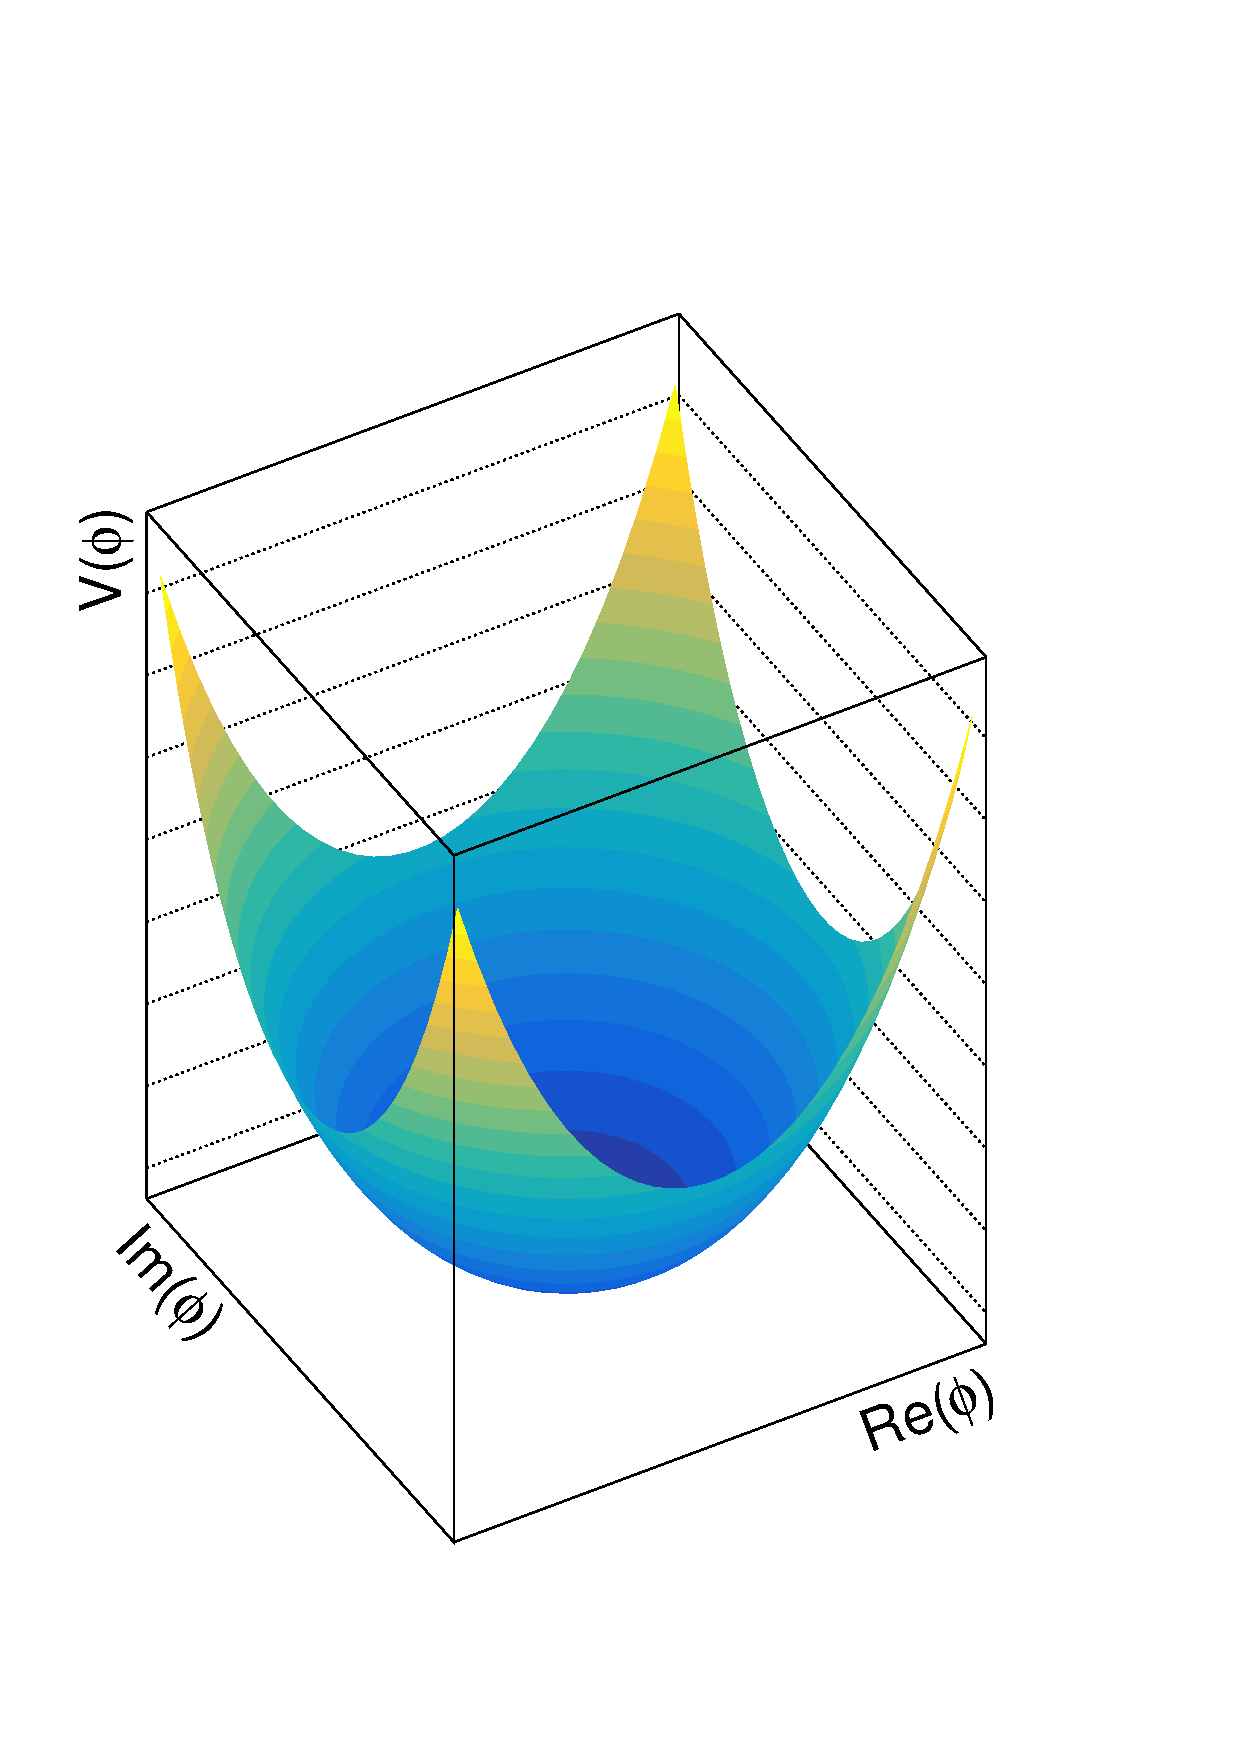
\includegraphics[width=0.49\textwidth]{produce_plots/sm/higgs_posmu2.pdf}\label{fig:sm:HiggsV_1}}
\subfigure[]{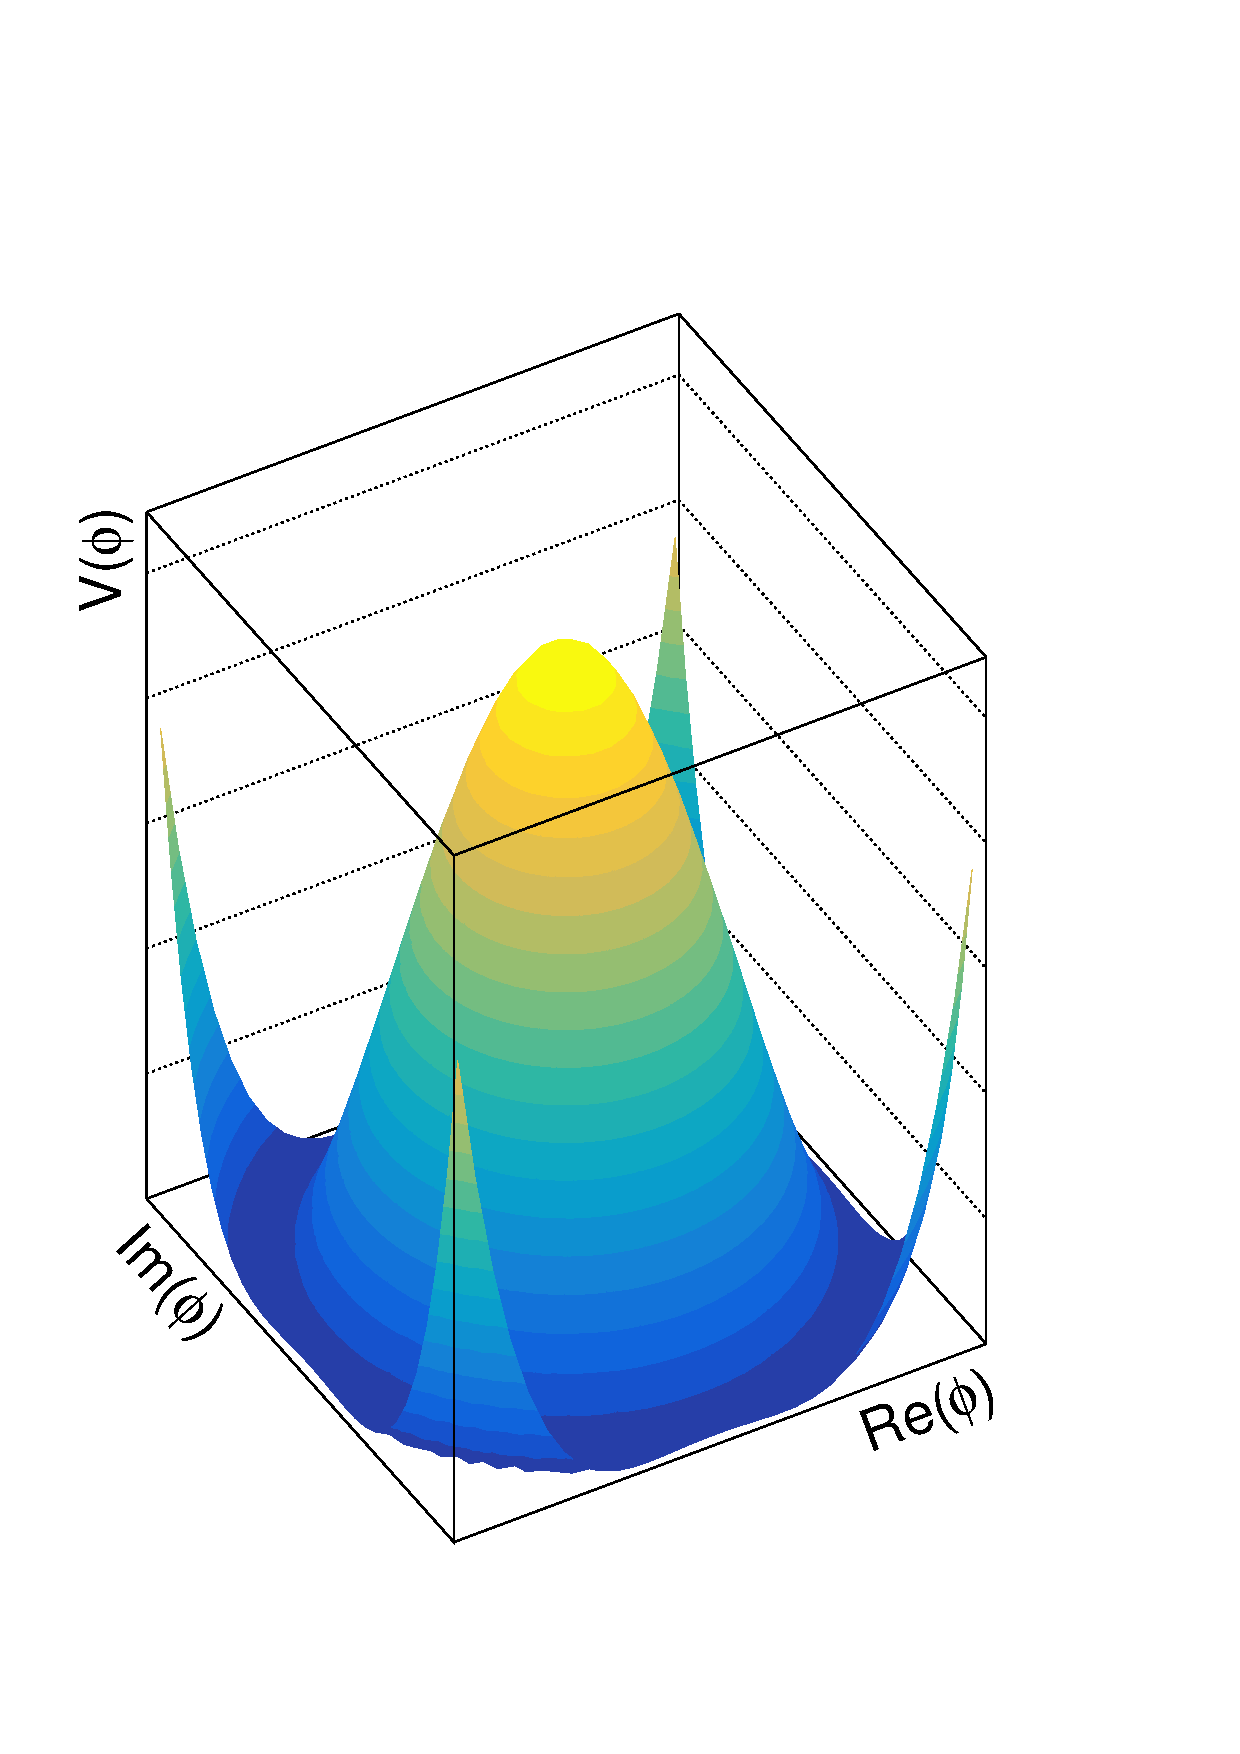
\includegraphics[width=0.49\textwidth]{produce_plots/sm/higgs_negmu2.pdf}\label{fig:sm:HiggsV_2}}
\caption{Higgs potential in the case \subref{fig:sm:HiggsV_1} $\lambda > 0$ and  $\mu^2 > 0$ and \subref{fig:sm:HiggsV_2} $\lambda > 0$ and $\mu^2 < 0$.}
\label{fig:sm:HiggsV}
\end{figure}

Up to this point the $SU(2)_\mathrm{L} \times U(1)_\mathrm{Y}$ symmetry is still intact, but the explicit choice of one of the infinite possible vacuum states for the Higgs field breaks the symmetry. According to the Goldstone theorem \cite{Goldstone:1962es}, the breaking of a continuous symmetry leads to the appearance of new massless scalar particles as field excitations. These new degrees of freedom are absorbed by the existing gauge bosons, thus giving them mass. To meet the experimental requirement of a massless photon, the choice of the Higgs vacuum has not to break the electromagnetic symmetry, $U(1)_{EM}$, so the component of the Higgs doublet that acquires a \gls{vev} is the neutral one:

\begin{equation}
	\Phi_0 = \frac{1}{\sqrt{2}} \left( \begin{array}{c} 0 \\ v  \end{array} \right) \, . \
\label{eq:hvphi}
\end{equation}

We can then expand the field $\Phi$ considering small excitations around the minimum:

\begin{equation}
	\Phi = \frac{e^{i \vec{\sigma} \cdot \vec{\theta}(x)/v }}{\sqrt{2}} \left( \begin{array}{c} 0 \\ v + \phi(x) \end{array} \right) \, ,
\label{eq:hvphi}
\end{equation}

\noindent where $\phi(x)$ is the physical field associated with the Higgs boson, $\vec{\sigma}$ the Pauli matrices and $\vec{\theta}(x)$ the three degrees of freedom absorbed to give masses to the $Z$ and $W^\pm$ bosons. Inserting Equation \ref{eq:hvphi} into Equation \ref{eq:LHiggs} relates the mass of the Higgs boson to the parameters in the potential:
\begin{equation}
m_H = \sqrt{- 2 \mu^2} = \sqrt{2 \lambda} v \; .
\label{eq:sm:Higgsmass}
\end{equation}

Since the numeric value of the $\mu^2$ and $\lambda$ parameters is not set, the theory does not predict a specific value for $m_H$. 
The physical mass eigenstates of the gauge bosons are a rotation of the interaction eigenstates, given by:

\begin{equation}
\begin{aligned}
W_\mu^\pm &= \frac{W_\mu^1 \mp W_\mu^2}{\sqrt{2}} \; , \\
A_\mu &= B_\mu \cos\theta_W + W^3_\mu \sin\theta_W \; ,  \\
Z_\mu &= W^3_\mu \cos\theta_W - B_\mu \sin\theta_W \; ,
\end{aligned}
\label{eq:wein}
\end{equation}

\noindent where we have introduced the Weinberg angle $\theta_W$ such that:
\begin{equation}
\tan\theta_W \equiv \frac{g'}{g} \; .
\end{equation}


The $(\mathcal{D}_{\mu} \Phi)^{\dagger} (\mathcal{D}^{\mu} \Phi)$ term in Equation \ref{eq:LHiggs} gives rise to the physical mass of the gauge bosons: once applied to the Higgs field, the covariant derivative in Equation \ref{eq:sm:covD} produces terms quadratic in the gauge fields, that we interpret as mass terms:

\begin{equation}
\mathcal{L}_{\Phi} = \left(1+\frac{\phi}{v}\right)^2 \,
\left\{ m_W^2\, W_\mu^\dagger W^\mu
+ \frac{1}{2}\, m_Z^2\, Z_\mu Z^\mu \right\}\, +\, \mathcal{L}_H \; , 
\end{equation}

\noindent where $\mathcal{L}_H$ denotes all the terms in $\mathcal{L}_{\Phi}$ that involve only the Higgs field: Higgs boson mass, cubic and quadratic self-interaction. Note that the coupling of the gauge bosons with the Higgs field is proportional to the square of the boson mass.
At tree level the resulting masses of the gauge bosons are:

\begin{equation}
\begin{aligned}
m_\gamma &= 0 \; ,\\
m_Z &= \frac{v \sqrt{g^2 + g'^2}}{2} \; , \\
m_W &= \frac{vg}{2} =  \cos\theta_W m_Z \; .
\end{aligned}
\end{equation}


Therefore, the Higgs-Englert-Brout mechanism generates automatically a mass term for the gauge bosons, that does not break the global underlying $SU(2)_\mathrm{L} \times U(1)_\mathrm{Y}$ symmetry. The Higgs field is used also to make fermion mass terms arise, but in this case it is necessary to postulate a Yukawa interaction between the Higgs and fermion fields. The fermion masses are assumed to be proportional to the strength of the coupling and, unlike the masses of the gauge bosons, they are not related to other parameters of the theory. While the Higgs field itself is enough to give mass to down-type fermions, the mass term for the up-type fermions  requires the introduction of the complex conjugate of the Higgs field ($\Phi_C$):

\begin{equation}
 \Phi_C = i \sigma^2 \Phi^* 
	= i \left( \begin{array}{cc} 0 & -i \\ i & 0 \end{array} \right) 
	\left( \begin{array}{c} \phi^- \\ \phi^{0*} \end{array} \right)
	= \left( \begin{array}{c} \phi^{0*} \\ - \phi^- \end{array} \right) \; .
\end{equation}

\noindent If we identify as $y_f$ the coupling of the fermion $f$ to the Higgs field, referred to as Yukawa coupling, the additional part of the Lagrangian that generates the fermion masses is:

\begin{equation}
\begin{aligned}
\mathcal{L}_{Yukawa} &= - \left[  y_d \left( \bar{u}_L \,\, \bar{d}_L  \right) \Phi d_R +  y_u \left( \bar{u}_L \,\, \bar{d}_L  \right) \Phi_C u_R \right] + h.c. \\
&= - \frac{1}{\sqrt{2}} \left[  y_d \left( v + \phi \right) \bar{d}_L d_R + h.c. + y_u \left( v + \phi \right) \bar{u}_L d_u + h.c. \right]  \; .
\end{aligned}
\end{equation}

\noindent In this equation we can now easily identify the fermion mass terms, of the form:

\begin{equation}
m_f =  \frac{v}{\sqrt{2}} y_f \; .
\end{equation}

\noindent Note that, in the case of fermions, the coupling to the Higgs boson is directly proportional to the fermion mass. 
The matrices $y_f$ are not necessarily diagonal, but they can be diagonalized through a unitary transformation, which we can interpret as the transformation that relates the mass eigenstates to the weak interaction eigenstates. In the quark sector, this transformation is encoded in the \gls{ckm} matrix \cite{Cabibbo:1963yz, Kobayashi:1973fv}, that describes the mixing of the down-type quarks. In the \gls{sm} with three generations of fermions, the \gls{ckm} matrix is specified by three angles and one complex phase that provides the only source of CP violation.

\subsection{Measured properties of the Higgs boson}

The value of the Higgs boson mass is not predicted by the \gls{sm}, but it can be measured and, once it is know, the Higgs boson production cross-section and decay fractions can be predicted accurately. These predictions can be verified experimentally, providing hints toward believing that the discovered boson is indeed the \gls{sm} Higgs boson. In 2015 the ATLAS and CMS collaborations published a combined measurement of the Higgs boson mass \cite{Aad:2015zhl}:
\begin{equation}
m_H = 125.09 \pm 0.21 (\mathrm{stat.}) \pm 0.11 (\mathrm{syst.}) \;\; \mathrm{GeV}.
\end{equation}

\noindent This result uses the full Run 1 ATLAS and CMS data, analyzed in the $h \rightarrow \gamma \gamma$ and $h \rightarrow ZZ* \rightarrow 4 \; \mathrm{leptons}$ channels.


The discussion of the Higgs mechanism in Section \ref{sec:smsusy:ew} highlights interesting properties of the interactions involving the Higgs boson. In particular, the strength of its coupling with fermions and bosons is proportional respectively to the mass and the square of the mass of the particle involved. 
This is reflected on the \glspl{br}: they are high for the decay to particles with the highest mass that are kinematically allowed.
While the top quark mass is too large to have the decay $h \to t\bar{t}$, the large top Yukawa coupling leads to loop-induced couplings of the Higgs boson to massless particles (gluons and photons); these are of phenomenological interest as they lead to the main production mode (gluon-gluon fusion) and to the $h \to \gamma \gamma$ decay mode, which has a low \gls{br} but leads to a very clean signature and was one of the key channels for the Higgs boson discovery. 
%The theoretical \glspl{br} for a Higgs boson mass of 125.09 GeV are reported in Table \ref{tab:SMBranchingFractions}. 

%\begin{table}[htbp]
%\begin{center}
%\begin{tabular}{clcr@{\hskip 0.4ex}l} \\ 
%\hline
% &    Decay mode &\multicolumn{3}{c}{Branching fraction [\%]}  \\  \hline
% \hline
% &     $H \rightarrow b\bar{b}$       & &   $57.5$&${}\pm 1.9$    \\
% &     $H \rightarrow WW$       & &   $21.6$&${}\pm 0.9$   \\
% &     $H \rightarrow gg$       & &   $8.56$&${}\pm 0.86$  \\
% &     $H \rightarrow \tau \bar{\tau}$       & &   $6.30$&${}\pm 0.36$  \\
% &     $H \rightarrow c\bar{c}$       & &   $2.90$&${}\pm 0.35$  \\
% &     $H \rightarrow ZZ$       & &   $2.67$&${}\pm 0.11$  \\
% &     $H \rightarrow \gamma \gamma$       & &   $0.228$&${}\pm 0.011$  \\
% &     $H \rightarrow Zg$       & &   $0.155$&${}\pm 0.014$  \\
% &     $H \rightarrow \mu \bar{\mu}$       & &   ~~$0.022$&${}\pm 0.001$  \\ 
%\hline
%\end{tabular} 
%\end{center}
%\caption{Standard Model predictions for the decay \glspl{br} of a Higgs boson with a mass of 125.09~GeV, together with their uncertainties~\cite{Heinemeyer:2013tqa}. Table follows Ref. \cite{Khachatryan:2016vau}.}
%\label{tab:SMBranchingFractions}
%\end{table} 
The theoretical production cross-section and \glspl{br} for a Higgs boson with mass between 120 and 130 GeV are reported in Figure \ref{fig:sm:h_xsec_br}.

\begin{figure}[ht]
\centering
\subfigure[]{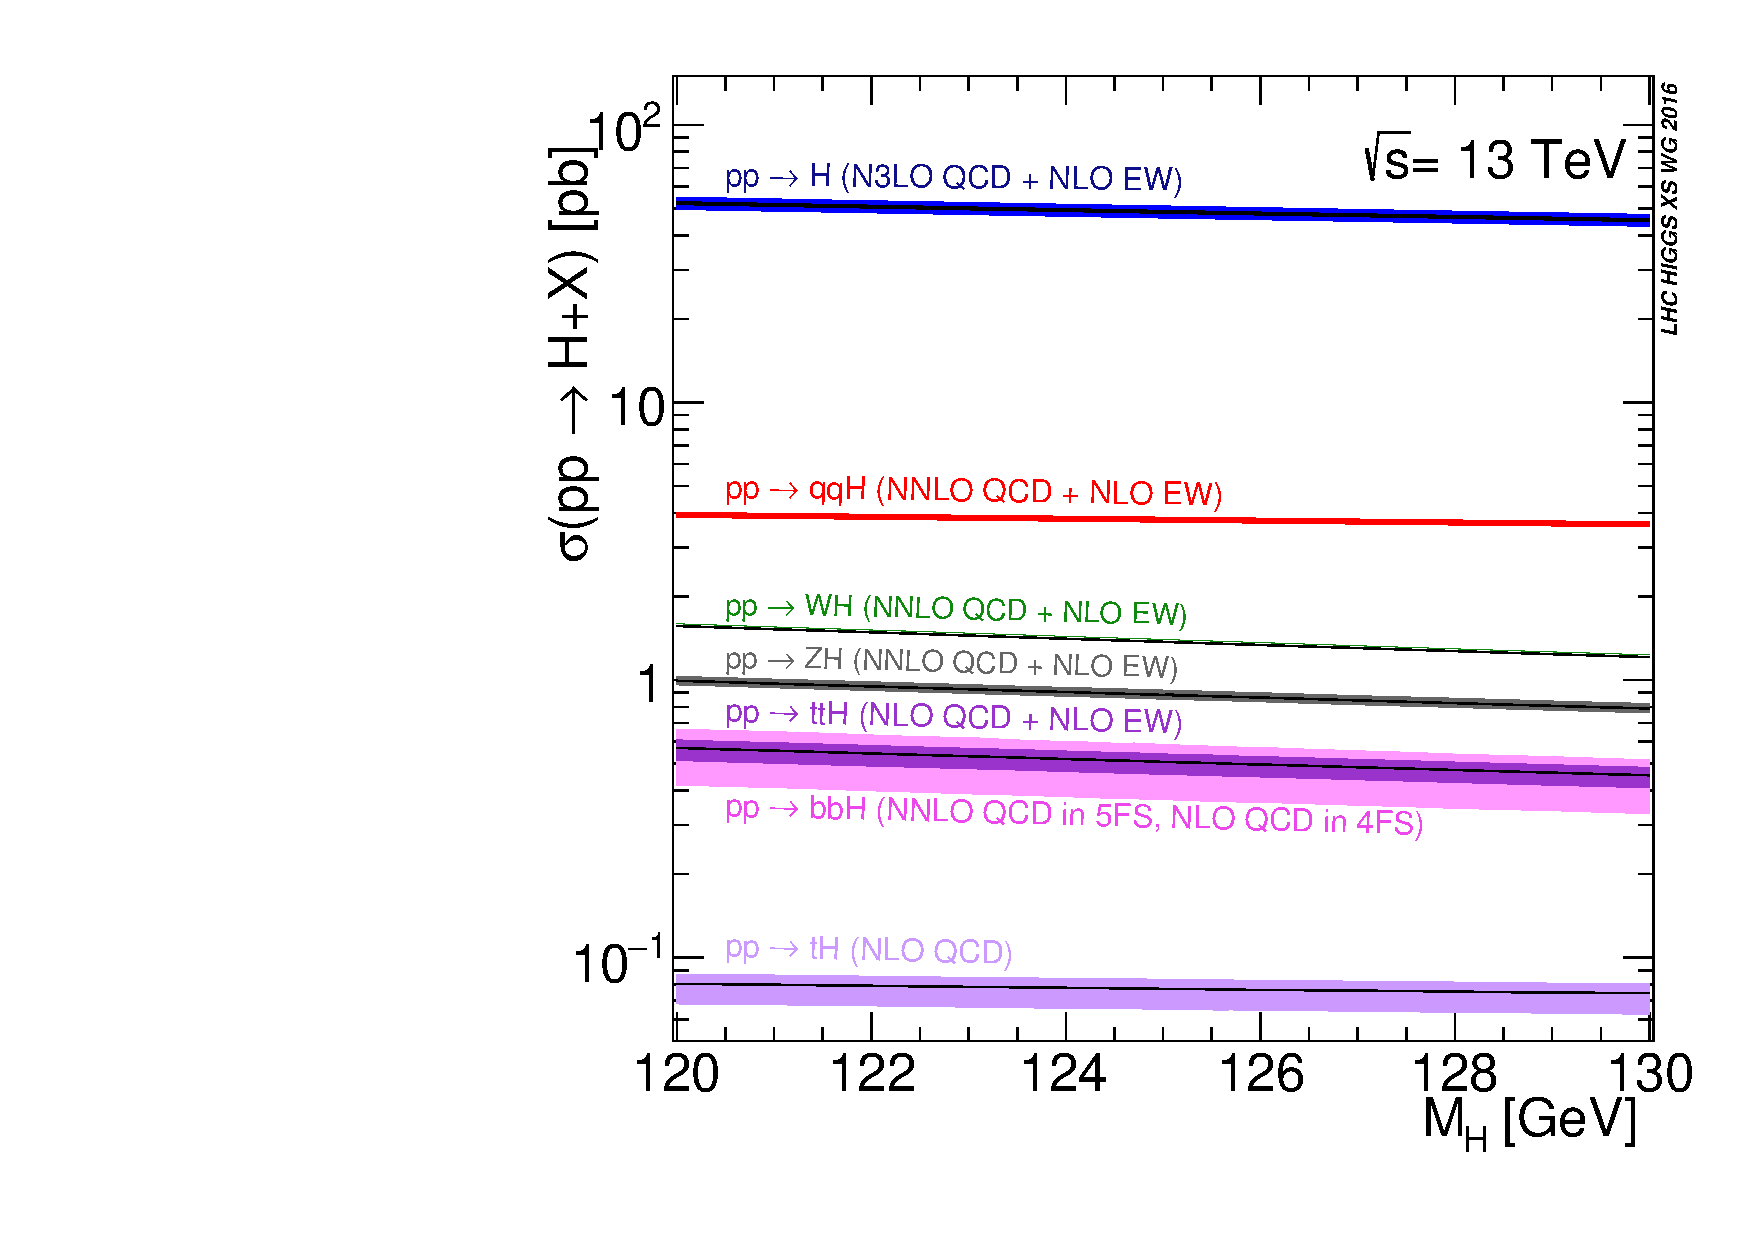
\includegraphics[width=0.49\textwidth]{figures/theory/plot_13tev_H_sqrt}\label{fig:sm:h_xsec_theo}}
\subfigure[]{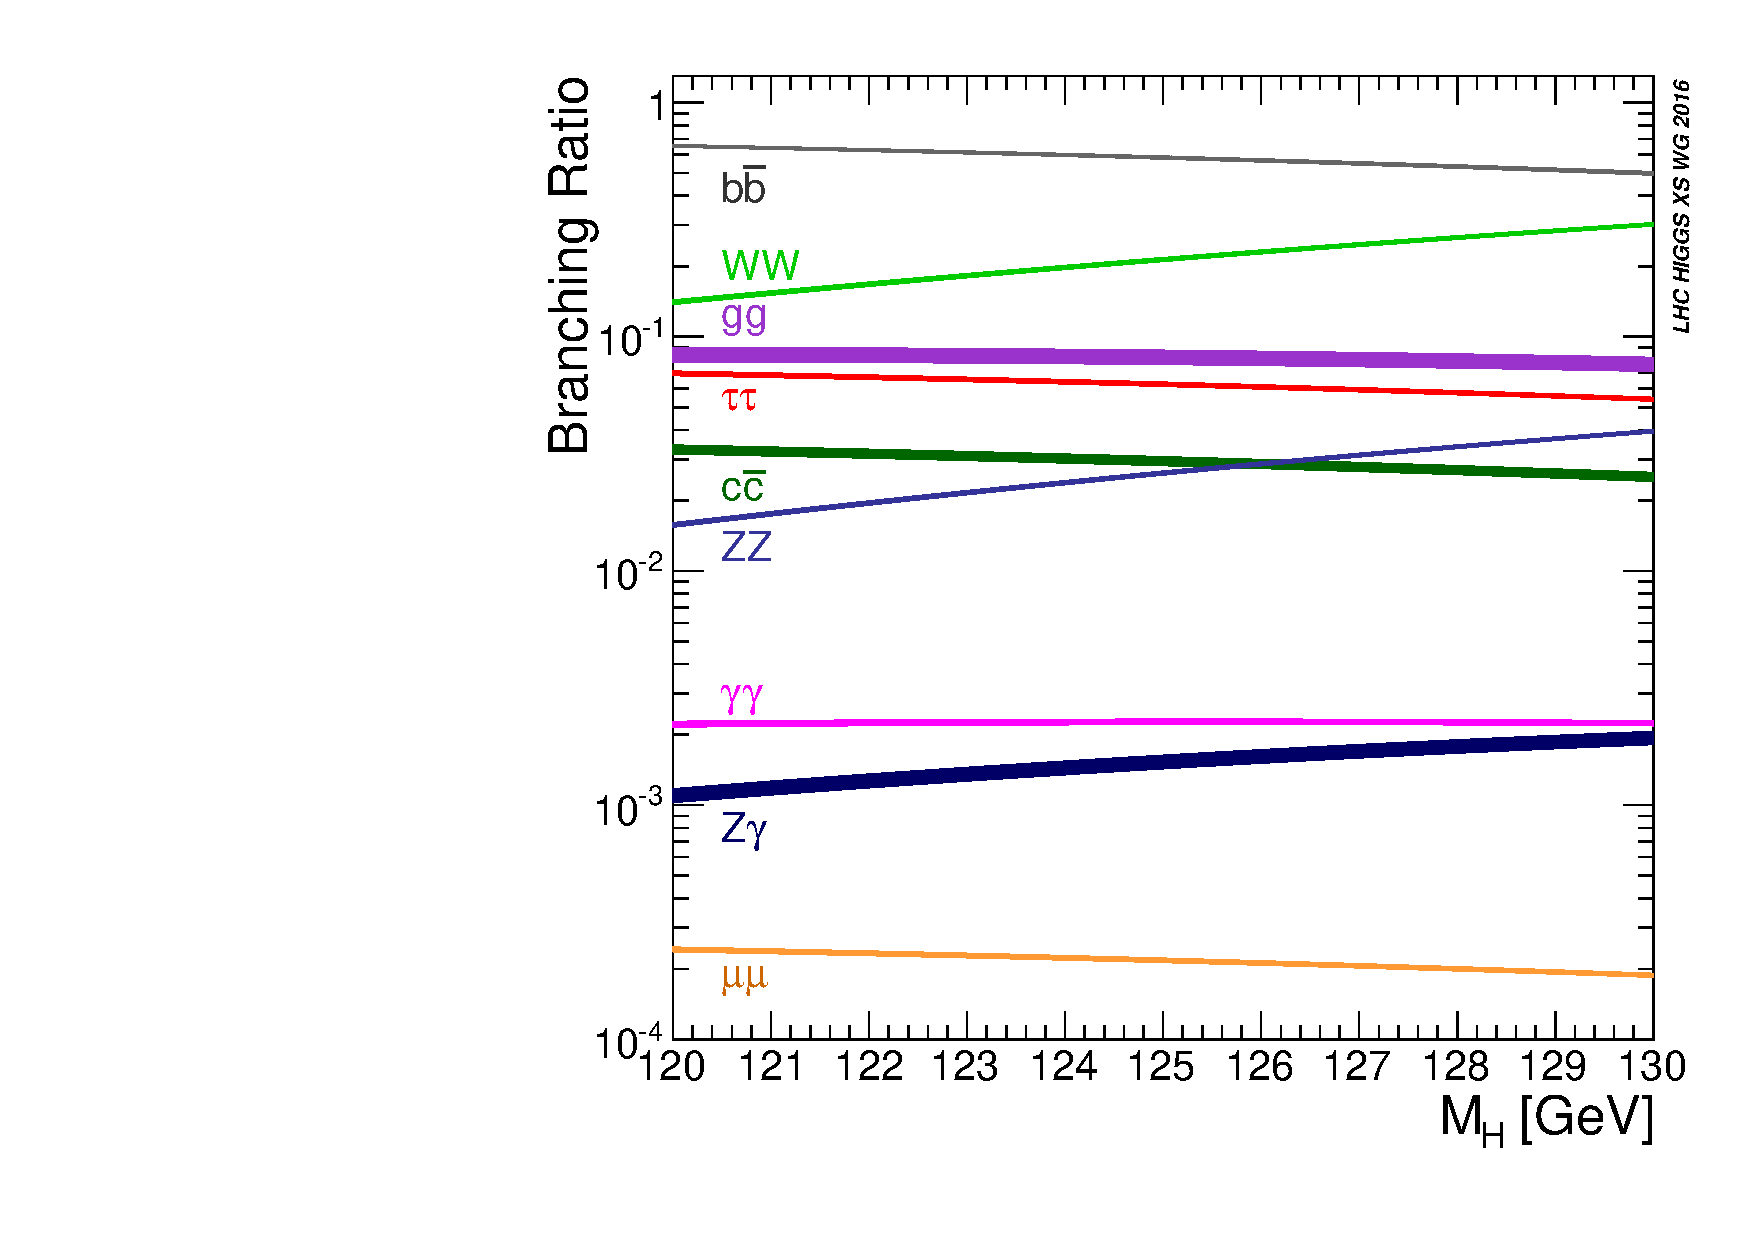
\includegraphics[width=0.49\textwidth]{figures/theory/SMHiggsBR_120-130.pdf}\label{fig:sm:h_br_theo}}
\caption{
\subref{fig:sm:h_xsec_theo} Higgs boson production cross-section at 13 TeV for a mass range between 120 and 130 GeV.
\subref{fig:sm:h_br_theo} Higgs boson \gls{br} for a mass range between 120 and 130 GeV.
Figures from Ref.  \cite{deFlorian:2016spz}.}
\label{fig:sm:h_xsec_br}
\end{figure}

The production cross-section is found to be in agreement with the \gls{sm} predictions within uncertainties. Figure \ref{fig:sm:h_xsec} shows the best fit value of Higgs production cross-section times \gls{br} in the different production and decay modes \cite{Khachatryan:2016vau}. Also the relation between the fermion or boson mass and the Higgs coupling has been verified experimentally, as show in Figure \ref{fig:sm:h_mass}. 

\begin{figure}[ht]
\centering
\subfigure[]{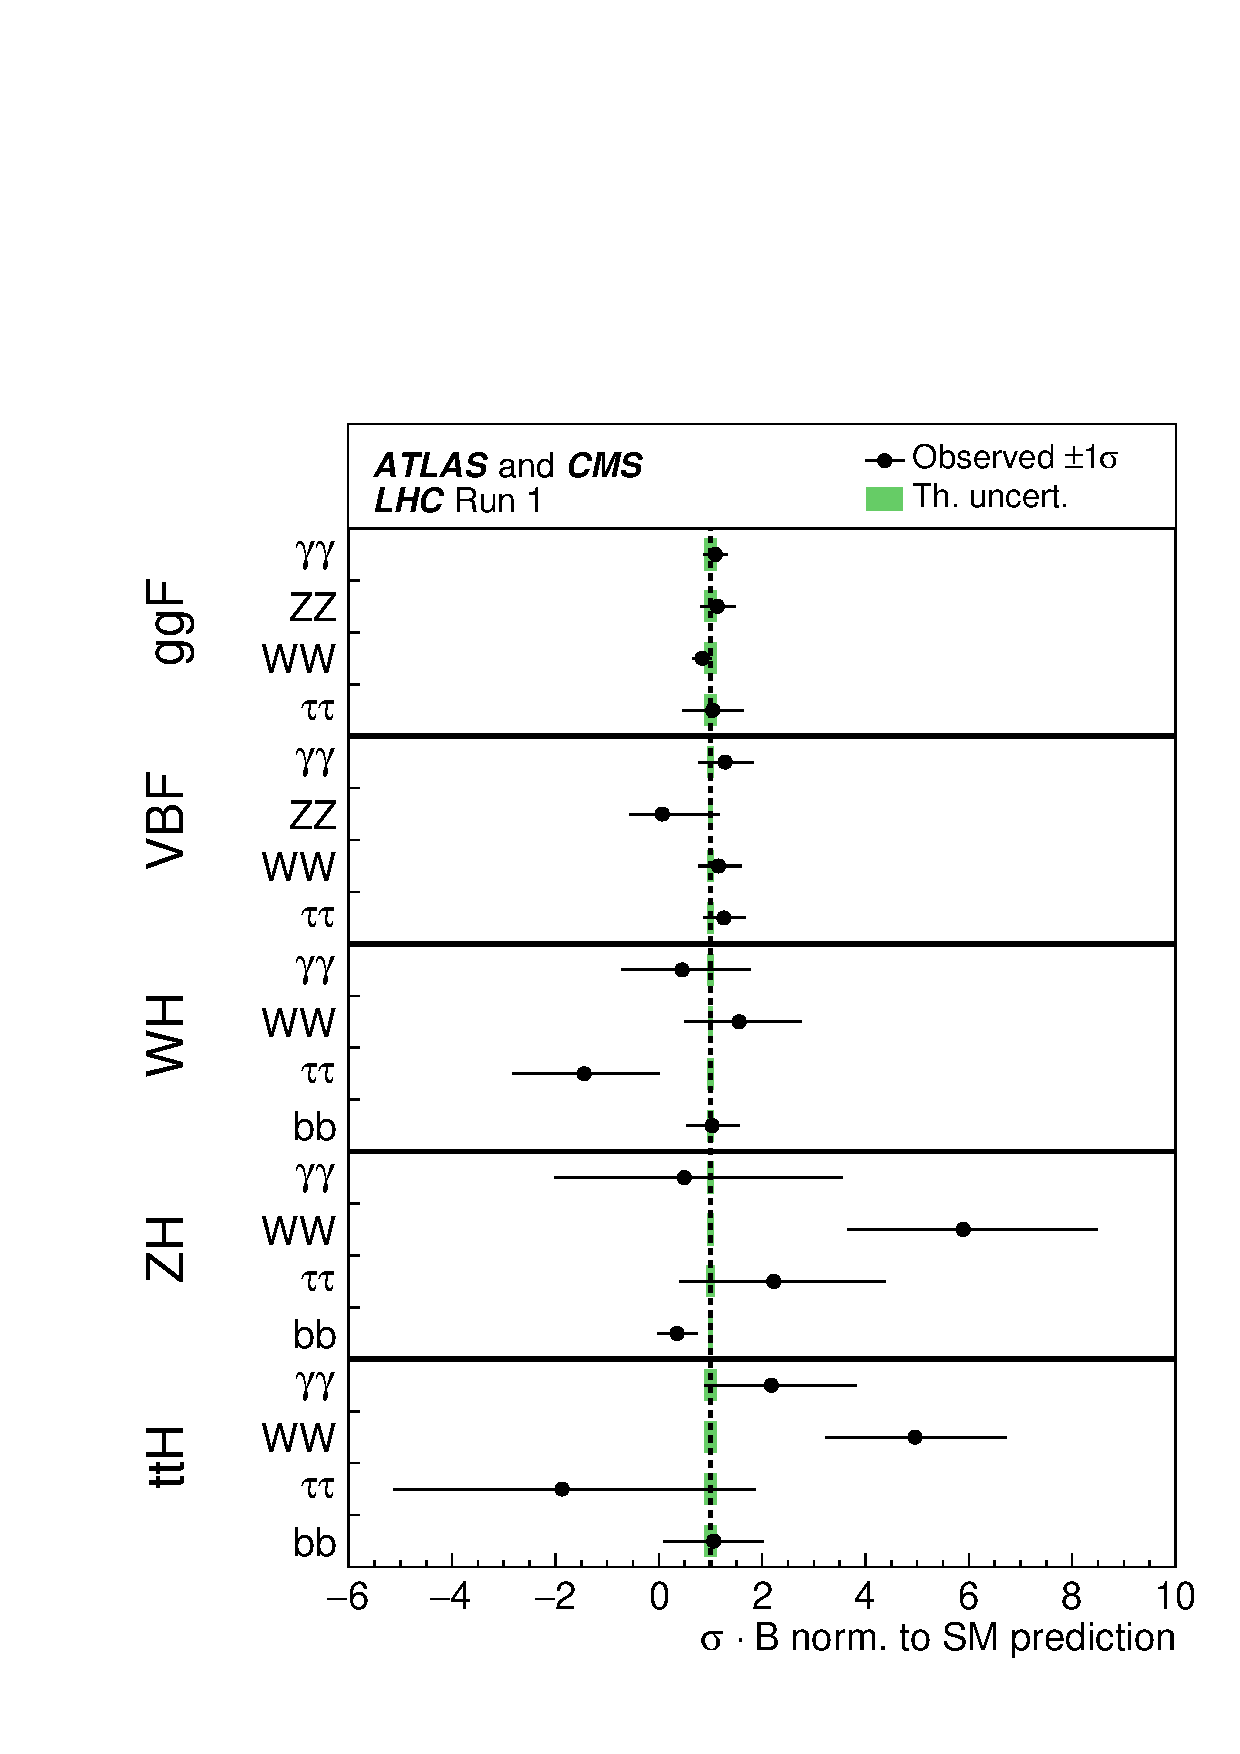
\includegraphics[width=0.49\textwidth]{figures/theory/CMS-HIG-15-002_Figure_007}\label{fig:sm:h_xsec}}
\subfigure[]{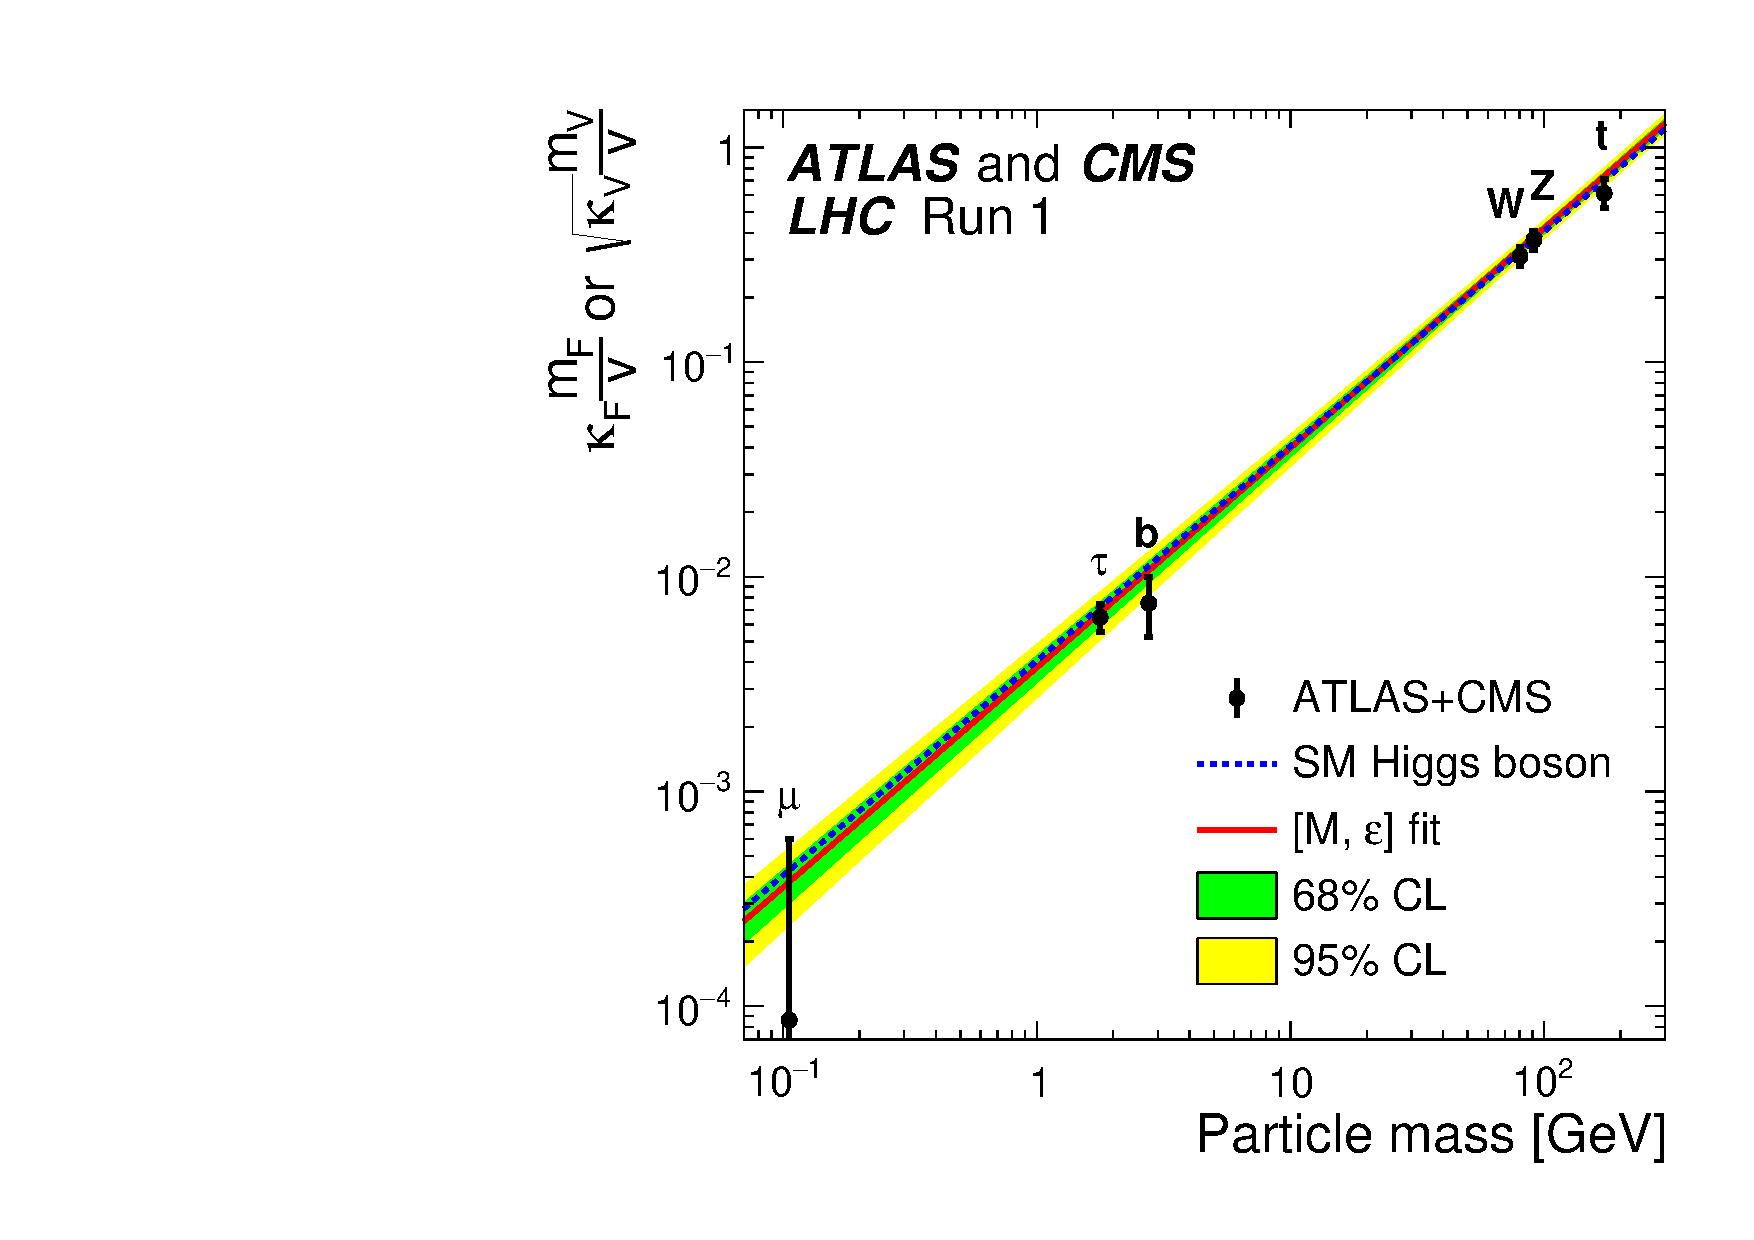
\includegraphics[width=0.49\textwidth]{figures/theory/CMS-HIG-15-002_Figure_019}\label{fig:sm:h_mass}}
\caption{\subref{fig:sm:h_mass} Best-fit values as a function of particle mass for the combination of Run 1 ATLAS and CMS data. \subref{fig:sm:h_xsec} Best-fit value of Higgs production cross-section times \gls{br} in different production and decay modes. Figure from Ref.  \cite{Khachatryan:2016vau}.}
\label{fig:sm:h_couplings_mass}
\end{figure}

 


\section{Limitations of the Standard Model and how to extend it}
\label{sec:smsusy:bsm}

Despite its undeniable success in describing the subatomic world, the \gls{sm} has some limitations that suggest it should be considered as the low-energy approximation of a more general theory. Nowadays there is no perfect candidate to fill the role of this general theory, but the shortcomings of the \gls{sm} highlight the characteristics this theory should have. Section \ref{sec:sm:missingpieces} discusses the experimental observations that are not accounted by the \gls{sm} framework, whose lacking is an objective limit of the \gls{sm}. In Section \ref{sec:sm:aesthetics} we review some other features that the \gls{sm} is missing that, while not being strictly necessary, would be desirable in a general theory. Some theories and models candidate to extend the \gls{sm} are briefly presented in Section \ref{sec:sm:extensions}.

\subsection{Unexplained phenomena}
\label{sec:sm:missingpieces}

The \gls{sm} lacks an explanation for some well established experimental phenomena that are listed in the next paragraphs.

\subsubsection*{Neutrino Masses}

Neutrino oscillations \cite{PhysRevLett.81.1562} are possible only if there is a mass difference between the three neutrino generations, which automatically implies non-zero masses for at least some neutrinos. Although neutrino mass terms could be accommodated by the \gls{sm} through right-handed neutrinos or a description of neutrinos as Majorana particles, the basic formulation of the \gls{sm} describes neutrinos as massless particles.

\subsubsection*{Dark Matter and Dark Energy}

The \gls{sm} describes only baryonic matter; this accounts for about 5\% of the energy density in the universe. Even though no direct observation of it has been made so far, we know there is also another type of matter, that does not have electromagnetic interactions and  is about five times more abundant than ordinary matter.  Since this type of matter does not reflect light, it is referred to as dark matter. The presence of dark matter has been postulated for the first time from the rotational velocity of galaxies \cite{Zwicky:1937zza}, but this evidence has now been confirmed also by other observations, including the analysis of the cosmic microwave background from the WMAP and Planck collaborations \cite{Larson:2010gs,Ade:2013zuv}. The sum of baryonic and dark matter accounts for about 32\% of the of the energy density in the universe. 
The remaining 68\%, known as dark energy, is the energy responsible for the accelerated expansion of the universe. While some extensions of the \gls{sm} provide candidates for dark matter, at the moment no theory provides a compelling explanation for dark energy.


\subsubsection*{CP Violation}

CP-violating processes are needed in order to generate the observed asymmetry between the matter and the anti-matter content of our universe. While the \gls{sm} provides one source of CP violation with the complex phase in the \gls{ckm} matrix mentioned in Section \ref{sec:smsusy:ew}, this is not enough and additional sources are needed in order to explain the observed asymmetry.

\subsubsection*{Gravity}

Gravity is the only force acting on elementary particles that is not described by the \gls{sm}. In fact, not only is not described by the \gls{sm}, but the simple attempt to quantize gravity through a spin-2  mediator (graviton) leads to a non-renormalizable theory. The strength of gravity is expected to be comparable to that of the other forces at the Planck scale ($\Lambda_{Planck}$, $\approx 10^{19}$ GeV). 

\subsection{Aesthetic shortcomings}
\label{sec:sm:aesthetics}

While the previous section discusses objective shortcomings of the \gls{sm}, there are also some aesthetic criteria that the \gls{sm} does not seem to satisfy. These are mostly based on the concept of Naturalness: unless there is a good reason, the parameters of a "beautiful" theory should be all of the same order of magnitude, and a theory where instead the parameters are bound to assume very specific and different values (fine tuning) seems "unnatural". It is important to notice that this naturalness requirement is subjective, as well as the amount of fine tuning allowed for a theory to be considered natural.


\subsubsection*{Hierarchy Problem}

The expression for the mass of the Higgs boson in Equation \ref{eq:sm:Higgsmass} contains only the tree-level contribution. The proper computation should include the radiative contributions from all the particles that couple with the Higgs boson, directly or indirectly (see below). A fermion, whose Yukawa coupling leads to the interaction $-y_f \phi \bar{f} f$, will produce a correction to the Higgs boson mass with a divergent integral; this can be computed e.g. with a cut-off regularization, and in this case the resulting correction to the Higgs boson mass, shown in Figure  \ref{fig:sm:h_corr_fermion}, is:
\begin{equation}
\Delta m_H^2 \>=\>  
-{|y_f|^2\over 8 \pi^2} \Lambda_{UV}^2 + \mathcal{O}(\ln \Lambda_{UV} ) \; ,
\label{eq:divhf}
\end{equation}

\noindent where $\Lambda_{UV}^2$ is the cut-off scale, identified with the limit of validity of the theory. If we assume that no physics \gls{bsm} is present up to $\Lambda_{Planck}$, having corrections to the mass proportional to $\Lambda_{Planck}$ requires a fine tuning of the parameters of the order of $\frac{m_H}{\Lambda_{Planck}} \approx 10^{-17}$. This is due to the strong hierarchy of the scales involved (hierarchy problem) \cite{Weinberg:1975gm, PhysRevD.20.2619, PhysRevD.14.1667, tHooft:1979rat}. Since the correction to the mass is proportional to the Yukawa coupling of the fermion, it is clear that the most important correction is the one given by the top quark, whose Yukawa coupling is $y_t \approx 1$. % 0.996 

Despite this, it can still be argued that the appearance of the $\Lambda_{UV}$ divergence is connected more to the regularization scheme rather than to the theory itself. But even in this case, the value of 125 GeV for the Higgs boson mass remains difficult to justify. The \gls{sm} Lagrangian does not have any symmetry that prevents the Higgs boson to couple to new \gls{bsm} particles. If we assume the existence of a complex scalar that couples with the Higgs field through $ -y_S|\phi|^2 |S|^2$, the correction to the Higgs propagator, shown in Figure \ref{fig:sm:h_corr_scalar}, is given by:

\begin{equation}
\Delta m_H^2 \>=\> {y_S\over 16 \pi^2}
\left [\Lambda_{UV}^2 - 2 m_S^2
\> {\rm ln}(\Lambda_{UV}/m_S) + \ldots
\right ] \; .
\label{eq:divhs}
\end{equation}

\noindent Beside the first term, proportional to $\Lambda_{UV}^2$, that can be thought as a consequence of the cut-off regularization, we also have a second  term proportional to $m_S^2$. If we assume that \gls{bsm} physics exists and that, since it has not yet been observed, $m_S$ must be large, this contribution drives $m_H$ to high values. A similar argument applies even if the new \gls{bsm} sector and the Higgs field do not couple directly but, for example, share a gauge interaction.

\begin{figure}[ht]
\centering
\subfigure[]
{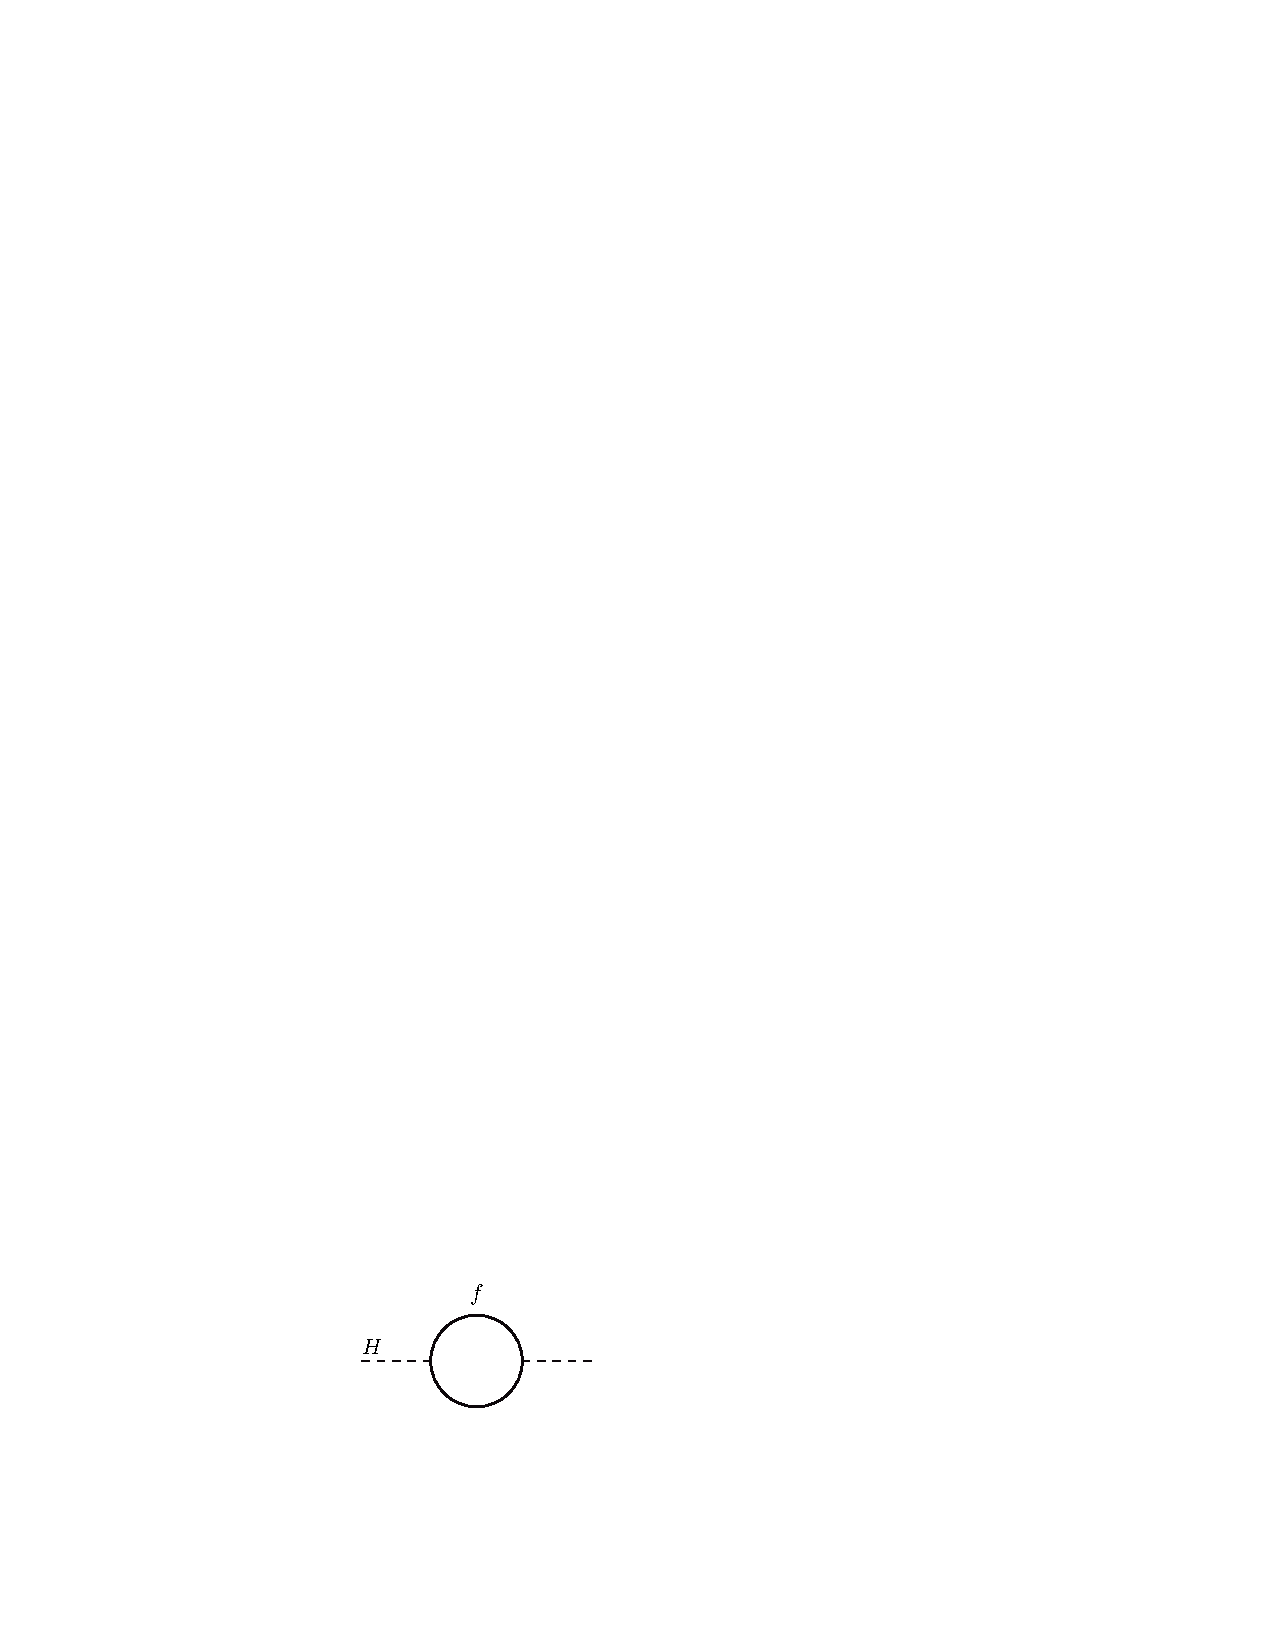
\includegraphics[width=0.36\textwidth]{figures/theory/h_corr_f.pdf}\label{fig:sm:h_corr_fermion}}
\subfigure[]{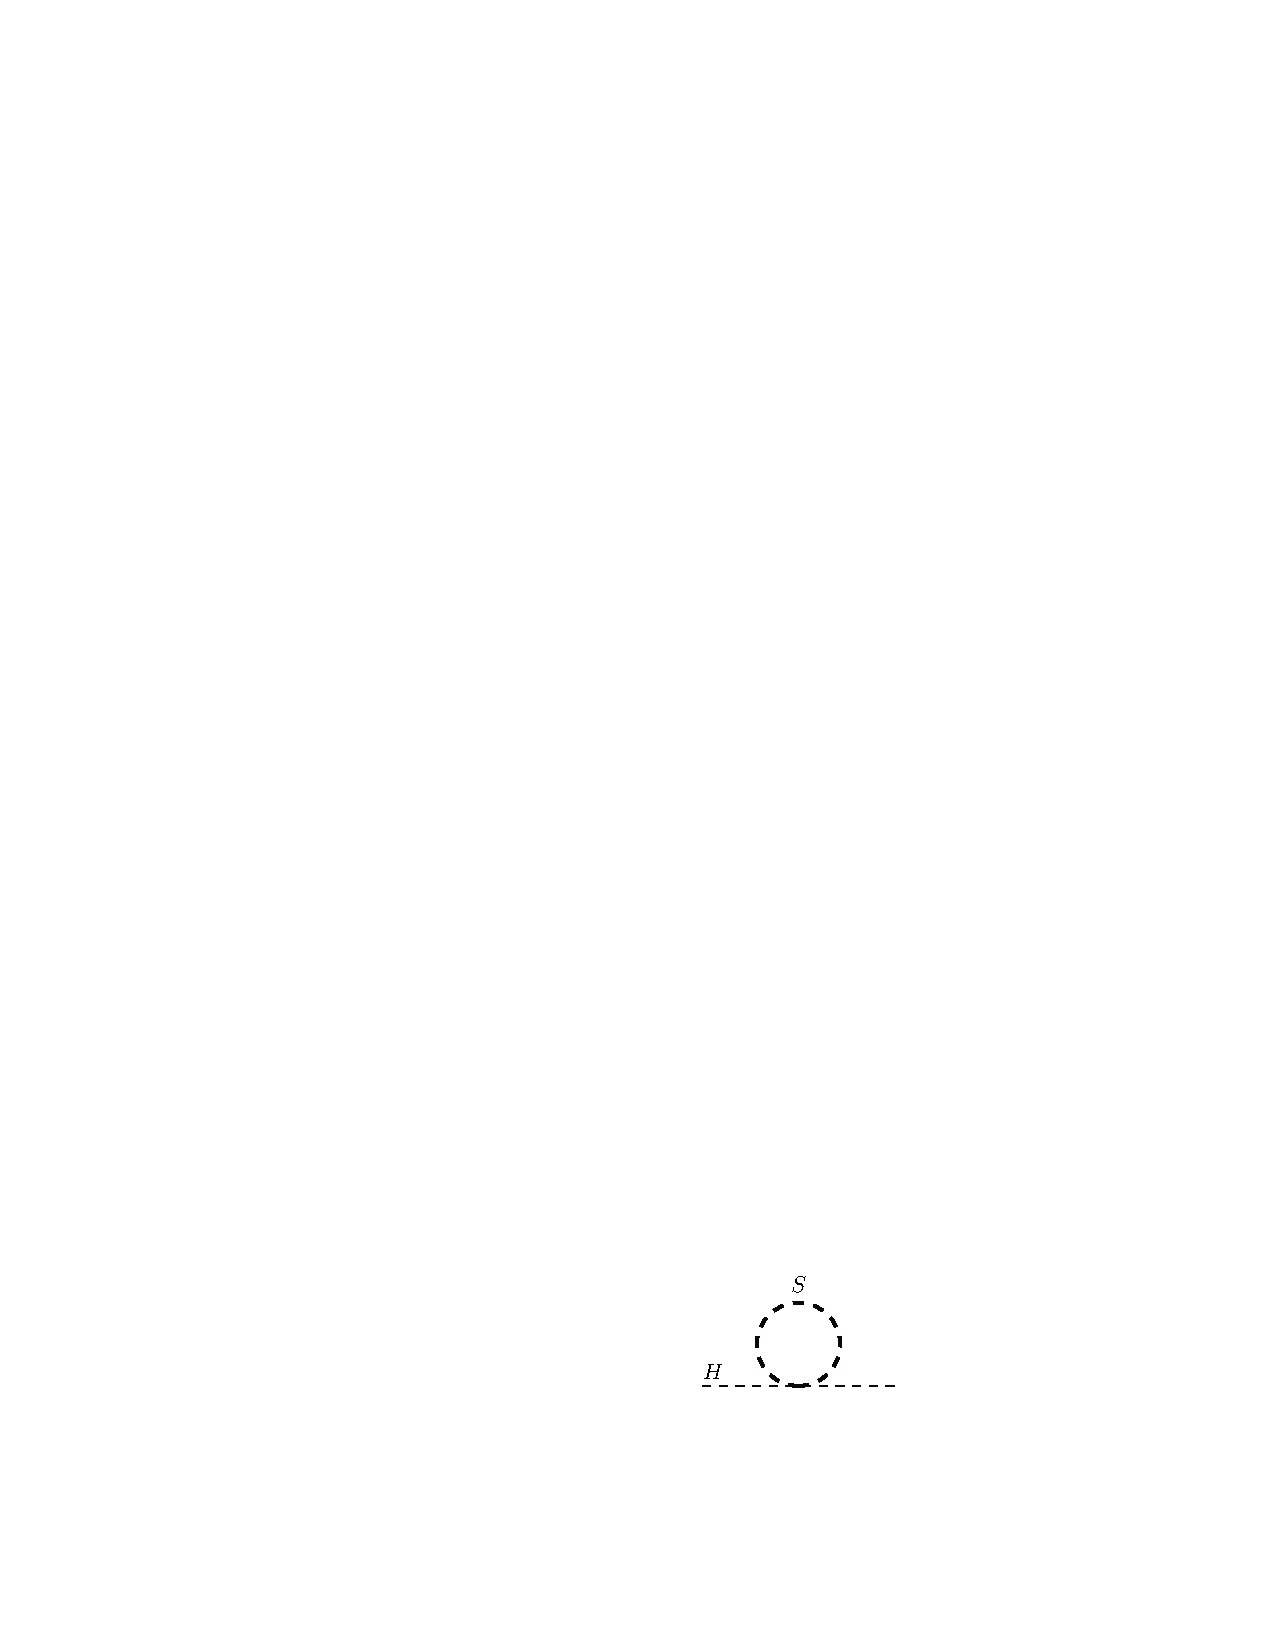
\includegraphics[width=0.36\textwidth]{figures/theory/h_corr_s.pdf}\label{fig:sm:h_corr_scalar}}
\caption{Correction to the Higgs boson propagator form the interaction with \subref{fig:sm:h_corr_fermion} a fermion and \subref{fig:sm:h_corr_scalar} a scalar. Figure from Ref. \cite{Martin:1997ns}.}
\label{fig:sm:h_corr}
\end{figure}

\subsubsection*{Fermion Mass Hierarchy} 

Fermion masses are less sensitive than the Higgs boson mass to the cut-off scale as the divergence is only logarithmic. Nevertheless, it is striking how strong the fermion Yukawa coupling hierarchy is: even if we don't consider neutrinos, fermion masses span about six orders of magnitude, without any apparent reason.

\subsubsection*{Unification of Coupling Constants}

The \gls{sm} coupling constants of the $SU(3)_\mathrm{C}$, $SU(2)_\mathrm{L}$ and $U(1)_\mathrm{Y}$ groups have a different evolution, and the extrapolation of their values at very high energies suggests a common value at a scale $M_{GUT} \approx 10^{15}-10^{16}$ GeV, after which the different couplings should unify. However, if the only particles involved in the computation of the evolution of the coupling constants are the \gls{sm} ones, there is no exact crossing point, as shown in Figure \ref{fig:susy:gut_0}.

\subsection*{Strong CP Problem}

The most general \gls{sm} \gls{qcd} Lagrangian should include also a CP-violating angle, and this would not spoil renormalizability. The presence of this term would have directly measurable physical consequences, for example a non-zero electric dipole moment for the neutron (nEDM). The tight  limits on the nEDM ( $< 3.6 \times 10^{-26}$ e cm at 95\% CL \cite{PhysRevD.92.092003}) translate into upper limits on the parameter regulating the CP-violating term of the \gls{qcd} Lagrangian ($\theta < 10^{-10}$ rad), while there is no theoretical reason why it should not be of order 1. 


\subsection{Extensions of the Standard Model}
\label{sec:sm:extensions}

The aspects of the particle physics world not yet described by the \gls{sm}, are an indication that the \gls{sm} should be extended.
In this section we briefly discuss a few of the most popular models proposed to extend the \gls{sm}, except from Supersymmetry which is discussed in more details in Section \ref{sec:smsusy:susy}. These extensions introduce typically one or more of the following:

\begin{itemize}
\item New particles, that can either be independent particles or "partners" of the \gls{sm} particles.
\item New symmetries, that can be broken. 
\item New degrees of freedom, such as new quantum numbers or extra dimensions.
\item New forces, whose strength depends on the energy scale.
\end{itemize}

\subsubsection*{Little Higgs}
% chiara: expand
Little Higgs models address the problem of the Higgs boson mass by considering the Higgs boson as a pseudo-Goldstone boson of a global symmetry \cite{PhysRevD.12.508, Kaplan:1983fs, KAPLAN1984187, DUGAN1985299}. This leads to a light mass for the Higgs boson is a similar way as for the pion in \gls{qcd}.

\subsubsection*{Technicolor}
In technicolor models \cite{Weinberg:1975gm, PhysRevD.20.2619} the mass of the $Z$ and $W^{\pm}$ bosons is not generated through the interaction with the Higgs boson, but dynamically with a new asymptotically free gauge interaction whose strength is higher at small distances; the analogy with \gls{qcd} (and the "color" degree of freedom) leads to the name technicolor. New fermions ("technifermions") are also introduced, transforming under the group vectorial representation. The Higgs boson is not predicted by technicolor, but it can be included in the model as a singlet scalar resonance, a dilaton, or a singlet pseudo-Goldstone boson.

\subsubsection*{Extra Dimensions}

The first attempt to introduce additional spacial dimensions to unify forces was done in the 1920's by Kaluza and Klein \cite{Kaluza, Klein:1926tv}, who interpreted our four-dimensional universe as a "brane" of a higher-dimensional space-time. While the \gls{sm} foresees only three spatial dimensions, adding extra dimensions can explain the observed weakness of gravity with respect to the other forces as it would be diluted in the extra dimensions. 
% rephrase
Particles propagating in the extra dimensions manifest in our brane as Kaluza-Klein modes. % end rephrase
While the original model from Kaluza and Klein was disproved shortly shortly after being proposed, similar ideas and formalism have also been used afterwards:  

\begin{itemize}
\item In the Arkani-Hamed-Dimopoulos-Dvali (ADD) model \cite{ArkaniHamed:1998rs}, two (or more) flat extra dimensions are added in which only gravity can propagate (through a graviton).
\item In the Randall and Sundrum model \cite{PhysRevLett.83.3370} the universe is conceived as a five-dimensional Anti-de Sitter space-time, and the weakness of gravity is explained through the red-shift of the gravity brane.
\end{itemize}


\section{Supersymmetry}
\label{sec:smsusy:susy}

\gls{susy} \cite{Wess:1974tw, Salam:1974ig} is an extension of the Poincar\'e group that rotates bosonic states into fermionic ones and vice versa, through the supercharge operator ($Q$) that carries itself a fermionic charge: 

\begin{equation}
\begin{aligned}
&Q |{\rm boson}\rangle = |{\rm fermion }\rangle \;, \\
&Q |{\rm fermion}\rangle = |{\rm boson }\rangle \; .
\end{aligned}
\end{equation}

\noindent The Haag-Lopuszanski-Sohnius extension of the Coleman-Mandula theorem \cite{HAAG1975257} allows such operator as the only non-trivial extension of the Poincar\'e group in a consistent four-dimensional theory, if the operator and his hermitian conjugate ($Q^\dagger$) satisfy the following relations:

\begin{equation}
\begin{aligned}
&\{ Q, Q^\dagger \} = P^\mu \; ,  \\
&\{ Q,Q \} = \{ Q^\dagger , Q^\dagger \} = 0  \;,  \\
&[ P^\mu , Q  ] = [P^\mu, Q^\dagger ] = 0 \; ,
\label{eq:susyalgth}
\end{aligned}
\end{equation}

\noindent where $P$ is the four-momentum operator. These relations, which define the Supersymmetry algebra, make it clear how the action of the supercharge is related to the Poincar\'e group: the combination of two Supersymmetry rotations is a space-time translation.

\subsection{Supermultiplets}

The irreducible representations of the \gls{susy} algebra are the supermultiplets, that contain both bosons and fermions. 
\gls{susy} particles are referred to as superpartners of the \gls{sm} particles within the same supermultiplet.
Superpartners of the \gls{sm} particles are indicated with the same symbol but with a $\sim$ on top of it. Depending on their particle content, supermultiplets are classified in different categories:

\begin{description}
\item[Chiral supermultiplets] These supermultiplets are the ones containing the \gls{sm} fermions and their superpartners. Each Dirac fermionic field can be regarded as two separate Weyl field, each of which has two degrees of freedom and is associated with a complex scalar as a superpartner. The name given to superpartners of fermions is sfermions (e.g. the superpartner of the top is the stop and the superpartner of the bottom is the sbottom). Since chiral supermultiplets are formed by spin-0 and spin-$\frac{1}{2}$ particles, they contain also the \gls{susy} extended Higgs sector, as described in Section \ref{sec:susy:Higgs}.

\item[Gauge supermultiplets] Gauge bosons and their superpartners belong to gauge supermultiplets. Each spin-1 \gls{sm} boson is associated to a spin-$\frac{1}{2}$ Weyl fermion, as before the electroweak symmetry breaking all the gauge bosons are massless and have only two degrees of freedom. The name of the superpartners of the gauge bosons is the same as the corresponding \gls{sm} particle but with a -ino suffix (e.g. the gluon superpartner is the gluino). 

\item[Gravitational supermultiplets] If we assume that gravity is mediated by the graviton, then a third type of supermultiplet is necessary that contains the spin-2 graviton and its superpartner, the spin-$\frac{3}{2}$ gravitino.

\end{description}

% Avoid fine tuning

% \gls{susy} is a broken symmetry


\subsection{Minimal Supersymmetric Standard Model}
\label{sec:theo:mssm}

\gls{susy} is a framework that allows to generate an infinite number of models. The \gls{mssm} is the one that allows to include and extend the \gls{sm} with the smallest number of extra parameters, and is based on the superpotential:

\begin{equation}
\begin{aligned}
W_{MSSM} & = y_u \stilde{u} \stilde{Q} H_u - y_d \stilde{d}\stilde{Q} H_d - y_e \stilde{e} \stilde{L}H_d + \mu H_u H_d \\  
& = \sum_{F, G, T} y_u^{FG} \stilde{u}_F \stilde{Q}_G^T H_u^T -
 = \sum_{F, G, T} y_u^{FG} \stilde{u}_F \stilde{Q}_G^T H_u^T - 
   \sum_{F, G, T} y_d^{FG} \stilde{d}_F \stilde{Q}_G^T H_d^T   \\ 
   & -
   \sum_{F, G, T} y_e^{FG} \stilde{e}_F\stilde{L}_G^T H_d^T  +
   \sum_{T} \mu H_u^T H_d^T \;.
\end{aligned}
\label{eq:WMMS}
\end{equation}

\noindent The superpotential appears in the \gls{mssm} Lagrangian through first and second order derivatives as discussed e.g. in Ref. \cite{Martin:1997ns}.

\begin{table}[t]
\begin{center}
\begin{tabular}{c c c c c}
\hline
\multicolumn{2}{c}{Names} 
& Spin 0 & Spin 1/2 & $SU(3)_C ,\, SU(2)_L ,\, U(1)_Y$
\\  \hline\hline
squarks, quarks & $Q$ & $({\stilde{u}}_L\>\>\>{\stilde{d}}_L )$&
 $(u_L\>\>\>d_L)$ & $(\>{\bf 3},\>{\bf 2}\>,\>{1\over 6})$
\\
($\times 3$ families) & $\bar{u}$
&${\stilde{u}}^*_R$ & $u^\dagger_R$ & 
$(\>{\bf \overline 3},\> {\bf 1},\> -{2\over 3})$
\\ & $\bar{d}$ &${\stilde{d}}^*_R$ & $d^\dagger_R$ & 
$(\>{\bf \overline 3},\> {\bf 1},\> {1\over 3})$
\\  \hline
sleptons, leptons & $L$ &$({\stilde{\nu}}\>\>{\stilde{e}}_L )$&
 $(\nu\>\>\>e_L)$ & $(\>{\bf 1},\>{\bf 2}\>,\>-{1\over 2})$
\\
($\times 3$ families) & $\bar{e}$
&${\stilde{e}}^*_R$ & $e^\dagger_R$ & $(\>{\bf 1},\> {\bf 1},\>1)$
\\  \hline
Higgs, higgsinos &$H_u$ &$(H_u^+\>\>\>H_u^0 )$&
$(\stilde{H}_u^+ \>\>\> \stilde{H}_u^0)$& 
$(\>{\bf 1},\>{\bf 2}\>,\>+{1\over 2})$
\\ &$H_d$ & $(H_d^0 \>\>\> H_d^-)$ & $(\stilde{H}_d^0 \>\>\> \stilde{H}_d^-)$& 
$(\>{\bf 1},\>{\bf 2}\>,\>-{1\over 2})$
\\  \hline
\end{tabular}
\caption{Chiral supermultiplets in the Minimal Supersymmetric Standard Model.
The spin-$0$ fields are complex scalars, and the spin-$1/2$ fields are 
left-handed two-component Weyl fermions. Table from Ref. \cite{Martin:1997ns}. \label{tab:chiral}}
\vspace{-0.6cm}
\end{center}
\par\bigskip
\begin{center}
\begin{tabular}{c c c c}
\hline
Names & Spin 1/2 & Spin 1 & $SU(3)_C, \> SU(2)_L,\> U(1)_Y$\\
\hline\hline
gluino, gluon &$ \stilde{g}$& $g$ & $(\>{\bf 8},\>{\bf 1}\>,\> 0)$
\\
\hline
winos, $W$ bosons & $ \stilde {W}^\pm\>\>\> \stilde {W}^0 $&
 $W^\pm\>\>\> W^0$ & $(\>{\bf 1},\>{\bf 3}\>,\> 0)$
\\
\hline
bino, $B$ boson &$\stilde{B}^0$&
 $B^0$ & $(\>{\bf 1},\>{\bf 1}\>,\> 0)$
\\
\hline
\end{tabular}
\caption{Gauge supermultiplets in
the Minimal Supersymmetric Standard Model. Table from Ref. \cite{Martin:1997ns}. \label{tab:gauge}}
\vspace{-0.45cm}
\end{center}
\end{table}

The chiral supermultiplets of the \gls{mssm} are described in Table \ref{tab:chiral}, and the gauge supermultiples in Table \ref{tab:gauge}. Note that the states defined in these tables are interaction eigenstates, but not necessary mass eigenstates as mixing is possible. In particular, the higgsinos mix with the gauginos to form neutralinos ($\stilde{\chi}^0_i$) and charginos ($\stilde{\chi}^\pm_i$). In addition, the sfermions associated with the left and right component of the same \gls{sm} fermion mix to form the sfermion mass eigenstates (e.g. $\stilde{t}_L$ and $\stilde{t}_R$ mix to form $\stilde{t}_1$ and $\stilde{t}_2$). The gluinos instead do not undergo any mixing, as there are no other superpartners with the same  quantum numbers. The gauge mass eigenstates of the \gls{mssm} are listed in Table \ref{tab:undiscovered}, assuming that the mixing within the first- and second-generation sfermions is negligible.


\begin{table}[tb]
\begin{center}
\begin{tabular}{c c c c c }
\hline
Names & Spin & $P_R$ & Gauge Eigenstates & Mass Eigenstates \\
\hline\hline
Higgs bosons & 0 & $+1$ & 
$H_u^0\>\> H_d^0\>\> H_u^+ \>\> H_d^-$ 
& 
$h^0\>\> H^0\>\> A^0 \>\> H^\pm$
\\ \hline
& & &${\stilde u}_L\>\> {\stilde u}_R\>\> \stilde d_L\>\> \stilde d_R$&(same)
\\
squarks& 0&$-1$& ${\stilde s}_L\>\> {\stilde s}_R\>\> \stilde c_L\>\>
\stilde c_R$& (same) \\
& & &
$\stilde t_L \>\>\stilde t_R \>\>\stilde b_L\>\> \stilde b_R$ 
&
${\stilde t}_1\>\> {\stilde t}_2\>\> \stilde b_1\>\> \stilde b_2$
\\ \hline
& & &${\stilde e}_L\>\> {\stilde e}_R \>\>\stilde \nu_e$&(same) 
\\
sleptons& 0&$-1$&${\stilde \mu}_L\>\>{\stilde \mu}_R\>\>\stilde\nu_\mu$&(same)
\\
& & &
$\stilde \tau_L\>\> \stilde \tau_R \>\>\stilde \nu_\tau$ 
&
${\stilde \tau}_1 \>\>{\stilde \tau}_2 \>\>\stilde \nu_\tau$
\\
\hline
neutralinos & $1/2$&$-1$ & 
$\stilde B^0 \>\>\>\stilde W^0\>\>\> \stilde H_u^0\>\>\> \stilde H_d^0$   
&
$\stilde \chi^0_1\>\> \stilde \chi^0_2 \>\>\stilde \chi^0_3\>\> \stilde \chi^0_4$ 
\\
\hline
charginos & $1/2$&$-1$ & 
$\stilde W^\pm\>\>\> \stilde H_u^+ \>\>\>\stilde H_d^-$ 
&
$\stilde \chi_1^\pm\>\>\>\stilde \chi_2^\pm $ 
\\
\hline
gluino & $1/2$&$-1$ &$\stilde g$  &(same) \\
\hline
${\rm goldstino}\atop{\rm (gravitino)}$ & ${1/2}\atop{(3/2)}$&$-1$&$\stilde 
G$  &(same) \\
\hline
\end{tabular}
\caption{The gauge and mass eigenstates of the \gls{mssm}. Table from Ref. \cite{Martin:1997ns}. 
\label{tab:undiscovered}}
\vspace{-0.4cm}
\end{center}
\end{table}%

Once the \gls{mssm} particles are introduced the computation of the evolution of the coupling constants, the unification of the forces discussed in Section \ref{sec:sm:aesthetics} is achieved, as shown in Figure \ref{fig:susy:gut_1}.

% Unifications of the coupling constants
\begin{figure}[ht]
\centering
\subfigure[]{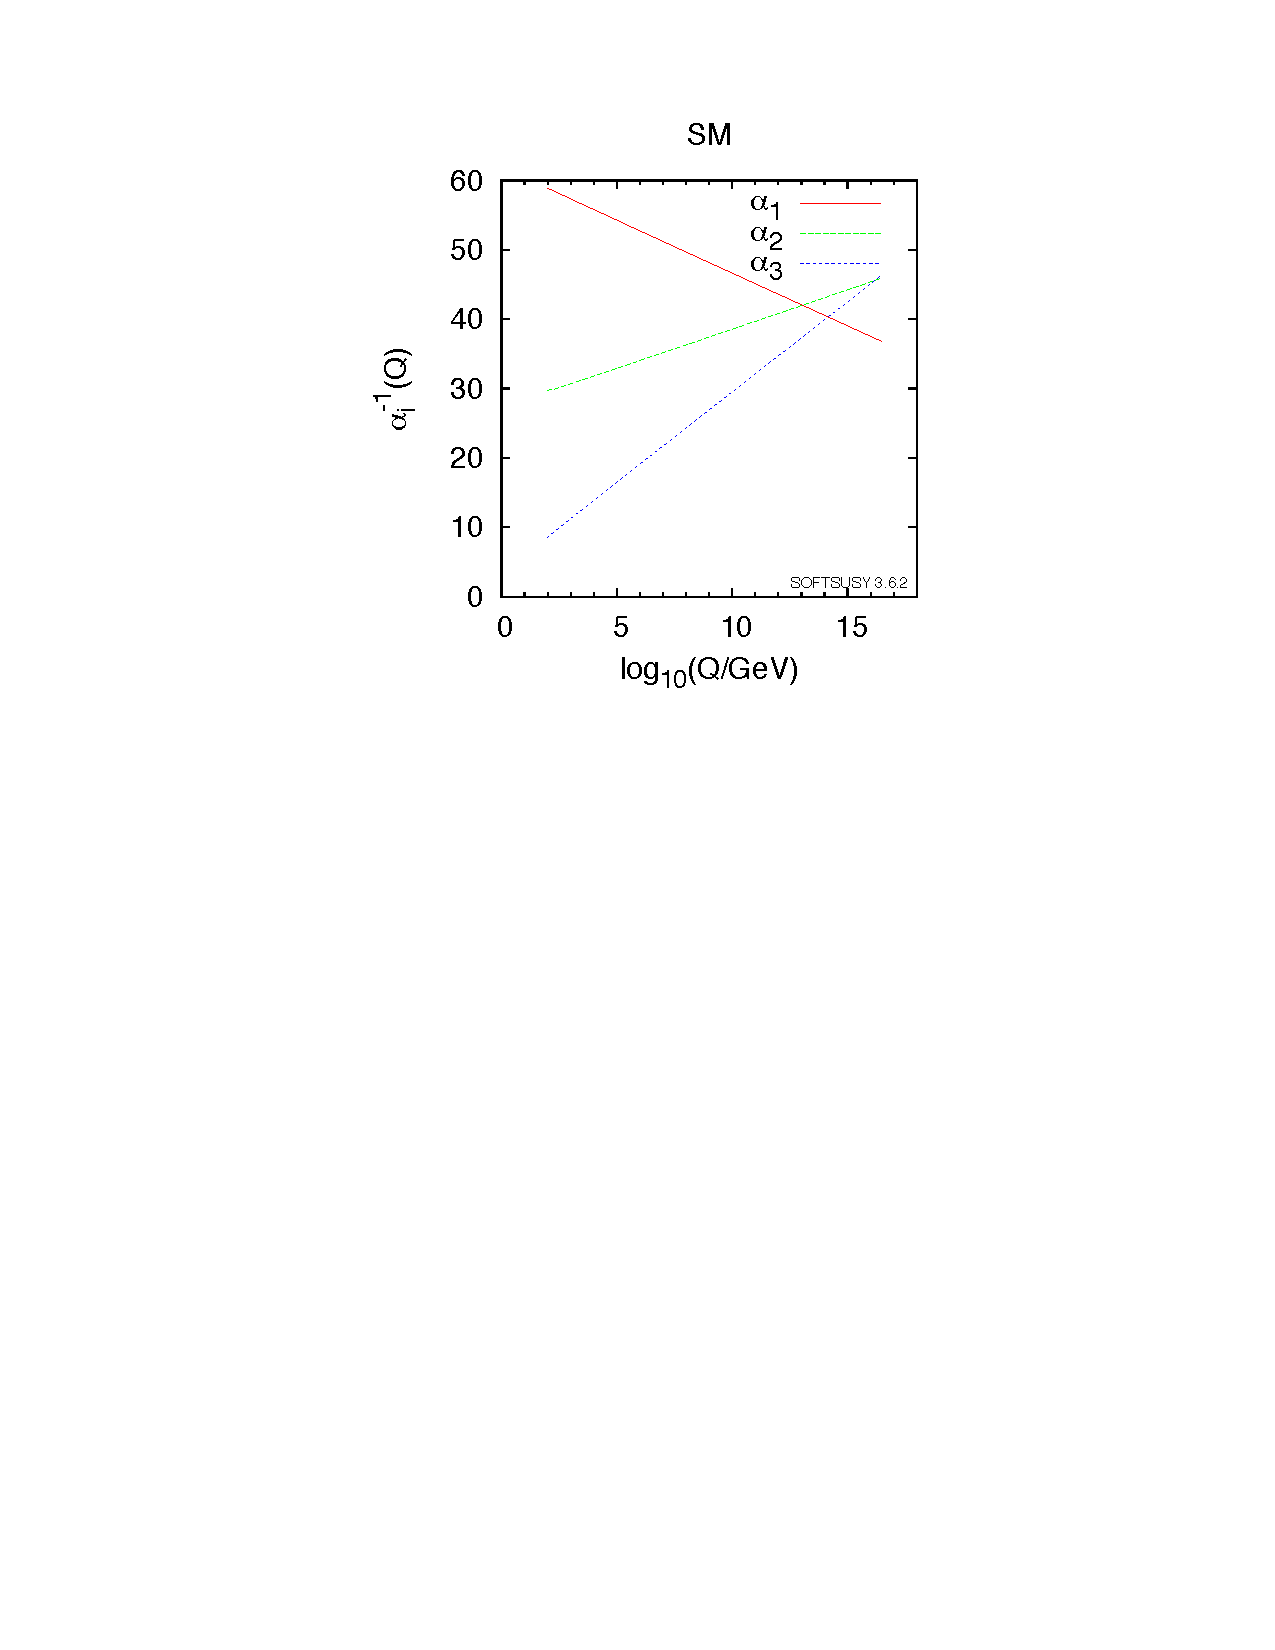
\includegraphics[width=0.45\textwidth]{figures/theory/gut_0.pdf}\label{fig:susy:gut_0}}
\subfigure[]{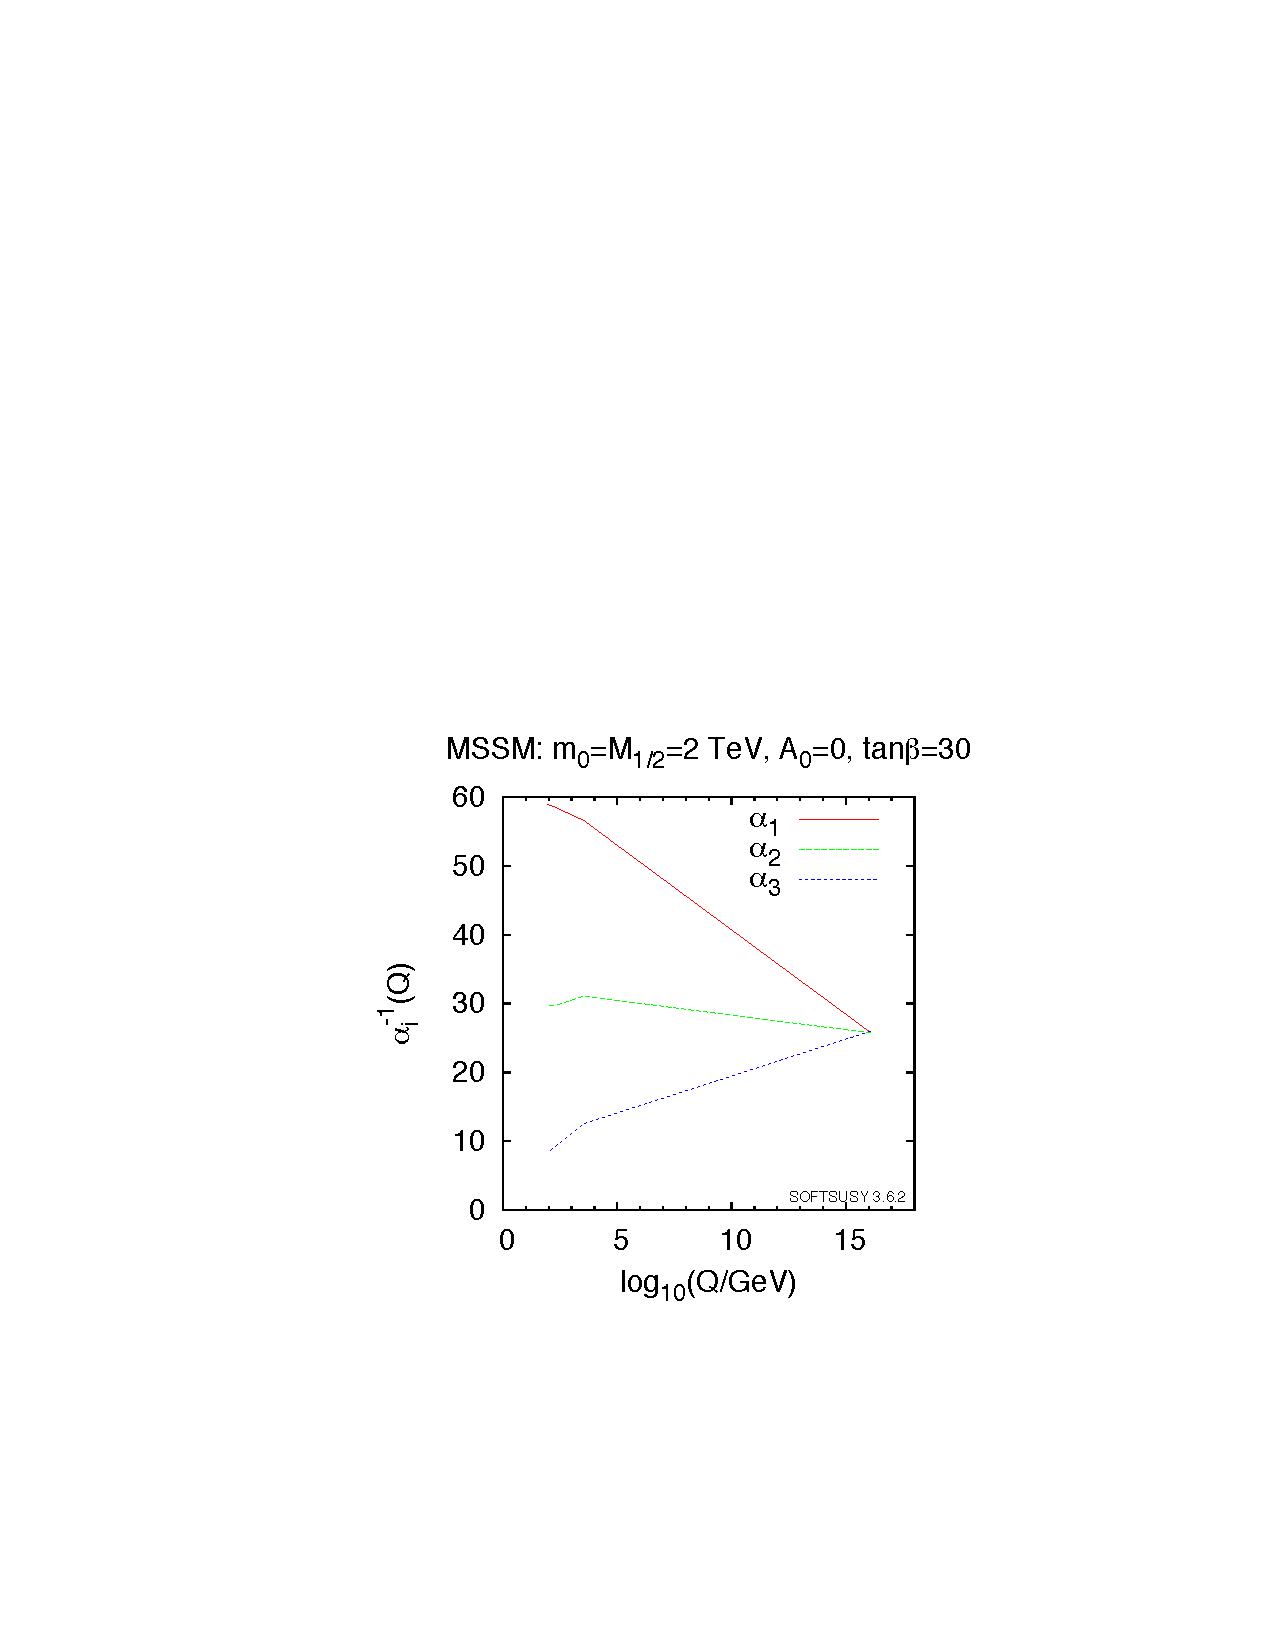
\includegraphics[width=0.45\textwidth]{figures/theory/gut_1.pdf}\label{fig:susy:gut_1}}
\caption{Evolution of the gauge couplings with energy scale in \subref{fig:susy:gut_0} the \gls{sm} and \subref{fig:susy:gut_1} the \gls{mssm}. Figure from Ref. \cite{Patrignani:2016xqp}.}
\label{fig:susy:gut}
\end{figure}

\subsubsection*{MSSM Higgs Sector}
\label{sec:susy:Higgs}

To maintain an holomorphic superpotential, \gls{susy} requires at least two SU(2) doublets: one to give mass to up-type quarks ($H_u$) and one to give mass to the the down-type quarks ($H_d$). The two doublets provide eight degrees of freedom. Three of them are  needed to give masses to the gauge bosons, while the other five become observable particles:
\begin{itemize}
\item Two CP-even neutral Higgs bosons: $h^0$ (the lighter) and $H^0$.
\item $A^0$, a CP-odd Higgs boson.
\item Two charged Higgs bosons, $H^+$ and $H^-$.
\end{itemize}


\subsubsection*{R-parity}

The \gls{mssm} does not include all the possible terms that are gauge- and \gls{susy}-invariant, to avoid interactions that would violate lepton or baryon number conservation. Matter parity, defined as:

\begin{equation}
P_M = (-1)^{3 (B-L)} \; ,
\label{eq:defmatterparity}
\end{equation}

\noindent is a multiplicative quantum number whose conservation implies automatically the conservation of lepton and baryon numbers (denoted with $L$ and $B$ respectively), without having to impose their conservation by hand. Particles in the same supermultiplet have the same matter parity: $P_M =-1$ for lepton and quark supermultiplets, while the Higgs and gauge supermultiplets have $P_M =+1$.

A more convenient way to express the same conservation rule is R-parity:

\begin{equation}
P_R = (-1)^{3(B-L) + 2 s} \; ,
\label{eq:defRparity}
\end{equation}

\noindent where $s$ is the spin of the particle. This is equivalent to matter parity as $(-1)^{2s}$ is conserved in all interactions where angular momentum conservation holds. The advantage of R-parity over matter parity is that for all \gls{sm} particles $P_R = 1$ and for all \gls{susy} particles $P_R=-1$. If  R-parity is conserved, in a collider experiment \gls{susy} particles are always produced in pairs, and each \gls{susy} particle always has an odd number of \gls{susy} particles in its decay products. As a consequence, the \gls{lsp} is stable; if the \gls{lsp} is electrically neutral, it interacts with ordinary matter mainly through gravity and thus it provides a good candidate for dark matter.

Note that R-parity conservation is not deduced from the theory and thus, while its consequences are appealing (especially the provision of a dark matter candidate), it is not an assumption that holds in all \gls{susy} models.



\subsection{Natural SUSY}
\label{sec:theo:naturalsusy}

Particles within the same supermultiplet share the same electric charge, isospin and \gls{qcd} color as $Q$ and $Q^\dagger$ commute with the generator of the gauge transformations.
The third equality in Equation \ref{eq:susyalgth} implies that $[ (P^\mu)^2 , Q  ]=0$. If we think of this as an operator applied to a supermultiplet, this implies that all the particles within the same supermultiplet should also have the same mass. The superpartners also bring a radiative correction to the Higgs boson mass, since they couple to the Higgs boson with the same coupling constant as their \gls{sm} partners ($y_S=y_f=y$). If we consider the case of a fermion and a sfermion, according to Eqs. \ref{eq:divhf}-\ref{eq:divhs} the two contributions have opposite sign and the total correction is:

\begin{equation}
\Delta m_H^2 \>=\> {y\over 16 \pi^2}
\left [ m_f^2
\> {\rm ln}(\Lambda_{UV}/m_f) 
- m_S^2
\> {\rm ln}(\Lambda_{UV}/m_S) 
\right ].
\label{eq:divhsusy}
\end{equation}

This correction cancels if each \gls{sm} particle and its superpartner have the same mass. Unfortunately we know that, if \gls{susy} exists, it must be a broken symmetry as the superpartners do not have the same mass as the corresponding \gls{sm} particles (otherwise they would have been already observed). Since the correction to the Higgs boson mass becomes larger with the increase of the mass difference between particles in the same supermultiplet, \gls{susy} remains a solution to the hierarchy problem as long as this mass difference is reasonably small. The term natural \gls{susy} refers to the class of \gls{susy} models that allow to solve (or mitigate) the fine-tuning problem that affects the Higgs boson mass; this has been a very active topic of discussion both before the start of the \gls{lhc} (see e.g. Refs. \cite{BARBIERI198863, Dimopoulos:1995mi}) and after (e.g. Refs. \cite{Papucci:2011wy, Casas:2014eca}) 

Not all the superpartners have the same relevance in the contribution to the Higgs-mass corrections, and a \gls{susy} model can be natural even if  most particles in it are extremely heavy. The particles that should be light in a natural \gls{susy} model are summarized in Figure  \ref{fig:NaturalSpectrum} and are:
\begin{itemize}
\item higgsinos, whose tree-level mass is directly controlled by the $\mu$ parameter,
\item stops, which contribute at one loop to the Higgs boson mass, and
\item gluinos, which contribute at two loops, since they give a one-loop correction to the stop mass.
\end{itemize}

% formula for relation between mass difference and correction to Higgs boson mass

%In the MSSM, the mass of the $Z$ boson and the Higgs sector masses are related at tree level through:
%\begin{equation}
%\label{eq:tune}
%-\frac{m_Z^2}{2} = |\mu|^2 + m_{H_u}^2.
%\end{equation}
%Where $\mu$ is the higgsino mass parameter and $m_{H_u}$ the mass term for the Higgs field that gives mass to down-type quarks. While \ref{eq:tune} holds only at tree level, it still means that if the masses of the superpartners in the Higgs sector are too large, fine-tuned loop corrections will be required to bring the left side of the equation down to the observed value of the $Z$-boson mass.

%\begin{equation}
%\Delta \equiv \frac{2\delta m_{H}^{2}}{m_{h}^{2}}.
%\end{equation}
% Z mass at tree level and definition of fine tuning

% susy particles that have to be light 

\begin{figure}[h!]
\begin{center} 
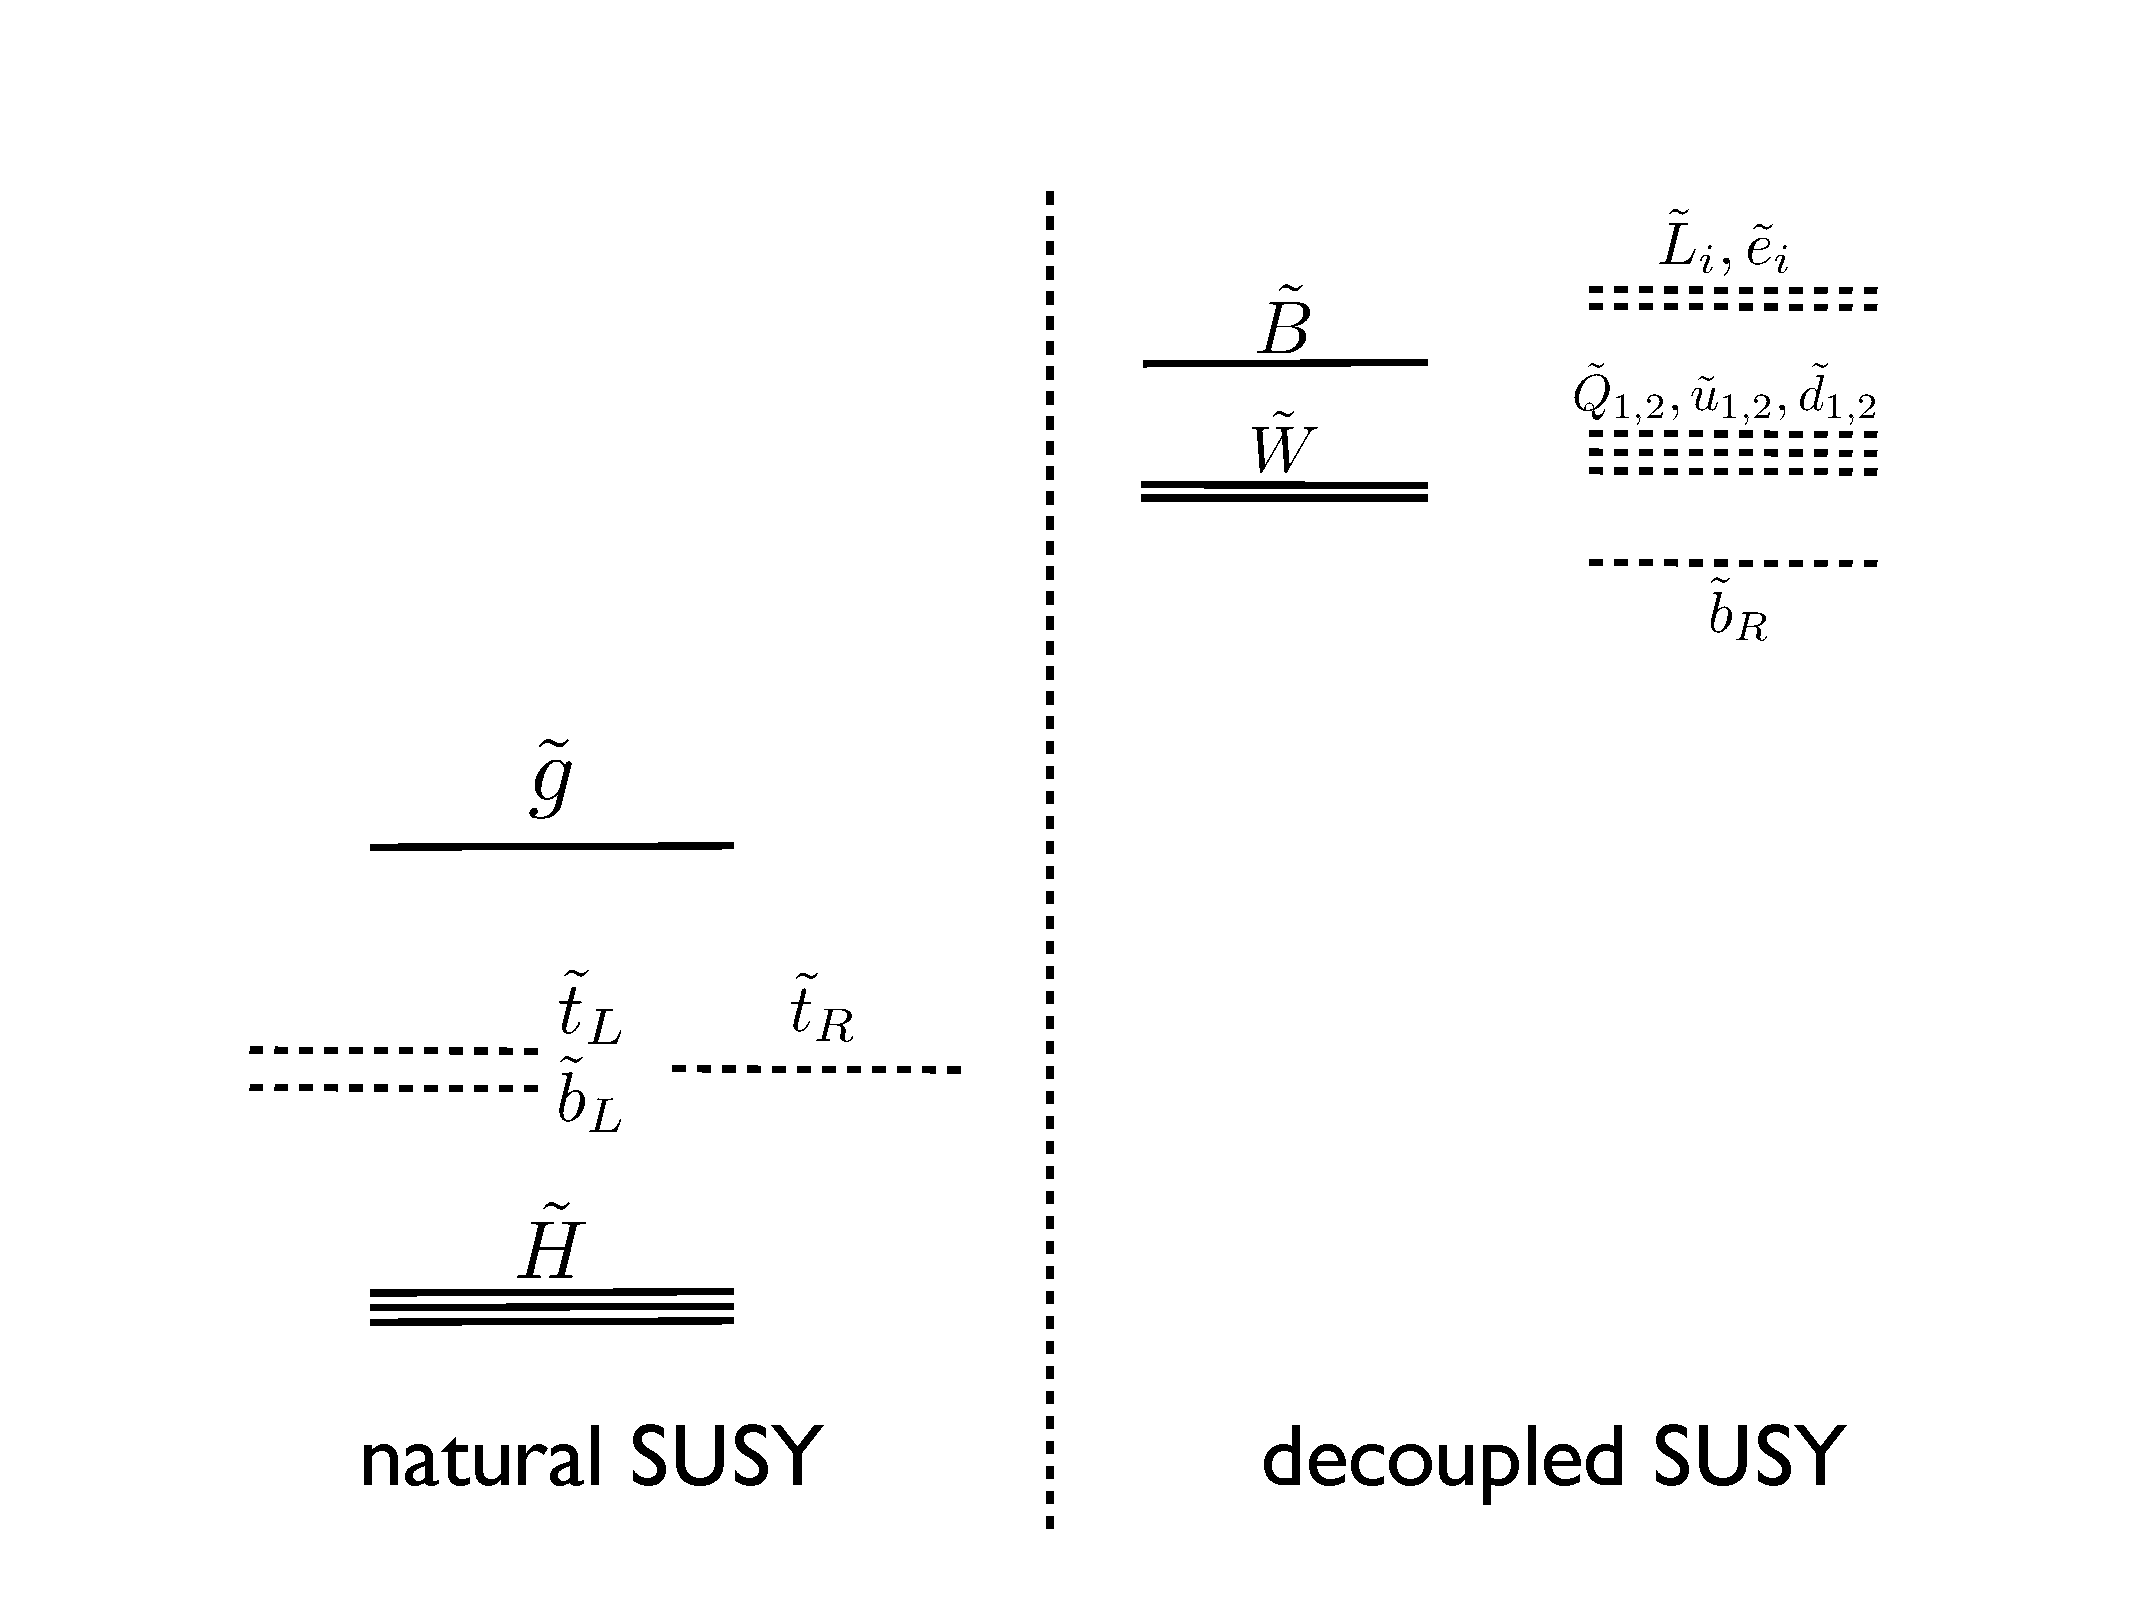
\includegraphics[width=0.8\textwidth]{figures/theory/NaturalSpec.pdf} 
\end{center}
\caption{The Naturalness argument constrains the masses of the \gls{susy} particles on the left side of the figure to be light, while the superpartners on the right side of the figure can have arbitrary mass without spoiling the Naturalness of the model. Figure from Ref. \cite{Papucci:2011wy}.}
\label{fig:NaturalSpectrum}
\end{figure}


\subsection{SUSY breaking in the MSSM}

Superpartners of the \gls{sm} particles have not been observed yet. This means that, if they exist, their mass must be larger than that of the corresponding \gls{sm} particle, and thus \gls{susy} must be a broken symmetry. The Lagrangian can therefore be written as:

\begin{equation}
\lagr = \lagr_{\rm SUSY} + \lagr_{\rm soft} \; ,
\end{equation}

\noindent where $\lagr_{\rm SUSY}$ is the \gls{susy}-conserving part derived from the superpotential, while $\lagr_{\rm soft}$ encloses the terms that break \gls{susy}. The suffix "soft" means that we allow in the Lagrangian only soft \gls{susy}-breaking terms, whose couplings have positive mass dimension, so that they vanish at very high mass scales. The inclusion of \gls{susy}-breaking terms requires the addition of new particles and interactions to the \gls{mssm}. While there is no unambiguous way to modify the theory to do this (some examples of \gls{susy}-breaking mechanisms are described in Section \ref{sec:susybreaking}), it is possible to include in the Lagrangian a general parametric form of the \gls{susy}-breaking terms:
\begin{itemize}
\item Gaugino masses, which in the \gls{mssm} correspond to the bino, wino and gluino mass terms;
\item Non-holomorphic scalar squared masses, which add mass terms for squarks and sleptons and contribute to the Higgs potential;
\item Holomorphic scalar squared masses, that in the \gls{mssm} can be present only in a term like $b H_u H_d$;
\item Scalar cubic couplings.
\end{itemize}  

The necessary \gls{susy}-breaking part of the Lagrangian adds to the \gls{mssm} many free parameters: in total the \gls{mssm} has 105 parameters in addition to the \gls{sm} ones.


\subsection{SUSY-breaking mechanisms}
\label{sec:susybreaking}

The \gls{susy}-breaking terms of $\lagr_{\rm soft}$ can be generated in models where \gls{susy} is spontaneously broken. This is the case if, just like  for the electroweak symmetry breaking, the Lagrangian is \gls{susy}-invariant, but the vacuum state is not. As it happens with the Higgs mechanism, the spontaneous breaking of a symmetry implies the appearance of a massless Goldstone particle (goldstino, $\stilde{G}$) that, in the case of \gls{susy}, has to be a neutral Weyl fermion in order to have the same quantum numbers as the supercharge $Q$. To be massless and annihilate the fermion mass matrix, the goldstino field has to be proportional to:

\begin{equation}
 \stilde{G} \,=\, 
 \begin{pmatrix}
\langle D^a \rangle /\sqrt{2} \cr \langle F_i\rangle 
\end{pmatrix} \; ,
\label{explicitgoldstino}
\end{equation} 

\noindent where $D^a$ and $F_i$ are respectively the auxiliary real bosonic and complex fermion fields of the \gls{susy} Lagrangian, and $\langle \rangle $ denotes their vacuum expectation value. For Equation \ref{explicitgoldstino} to be non-trivial, at least one of the $D^a$ or $F_i$ has to have a non-zero \gls{vev}. This is related to the two possible mechanisms that lead to \gls{susy} breaking: via a $D$-term or an $F$-term. 
The Fayet-Iliopoulos mechanism \cite{Fayet:1974jb} allows to have a non-zero \gls{vev} for an auxiliary field $D$ by adding to the Lagrangian a term proportional to the auxiliary field itself, and with a coupling constant with the dimension of a squared mass:
\begin{equation}
\lagr_{\rm FI} \,=\, -\kappa D \; .
\end{equation}
With this mechanism it is however difficult to attribute properly masses to all the \gls{mssm} particles.
%This type of term is gauge-invariant only for abelian groups. 
%the hypercharge symmetry group $U(1)_Y$ is not eligible 

Another possibility is to assign a \gls{vev} to an $F$-term, with the O’Raifeartaigh mechanism \cite{ORaifeartaigh:1975nky}. Since in the \gls{mssm} there is not a good candidate to be a gauge singlet with a non-vanishing \gls{vev} for an $F$-term, this implies the addition of at least one set of chiral supermultiplets, such that $F_i$ is non-trivial for at least one of them. A realization of this is possible for example with three chiral supermupliplets $\Phi_i$ and a superpotential of the form:
\begin{equation}
W = -k \Phi_1 + m \Phi_2 \Phi_3 + {y\over 2} \Phi_1 \Phi_3^2 \;.
\label{oraif}
\end{equation}
The resulting scalar potential at tree level has a minimum for $\phi_2=\phi_3=0$ and independent of $\phi_1$ (where $\phi_i$ are the scalar fields in $\Phi_i$), while the one-loop corrections highlight a non-zero global minimum when also $\phi_1=0$. In the following we will consider only \gls{susy} breaking originating from the O’Raifeartaigh mechanism.


When \gls{susy} is treated as a local symmetry, it has to include also gravity, and the resulting theory is called supergravity. The gravity mediator is the spin-2 graviton, and its superpartner the spin-$\frac{3}{2}$ gravitino. The gravitino can be interpreted as the gauge field of \gls{susy}, and it incorporates the goldstino degrees of freedom upon spontaneous \gls{susy} breaking. Therefore, the gravitino is also indicated with the same symbol as the goldstino, $\stilde{G}$. By dimensional arguments, we can understand that the gravitino mass ($m_{3/2}$) has to be proportional to:

\begin{equation}
m_{3/2} \approx \frac{\langle F \rangle}{\Lambda_P} \; ,
\label{mgrav}
\end{equation}
\noindent where $\langle F \rangle$ is the \gls{vev} of the \gls{susy}-breaking $F$-term, as it has to vanish both if \gls{susy} is an exact symmetry and if the Planck scale is extremely high (and thus gravity is negligible). 

For any \gls{susy}-breaking mechanism, the \gls{mssm} soft term do not appear at tree level, but are generated through radiative corrections. \gls{susy} breaking happens in a hidden sector, while the \gls{mssm} particle live in the visible sector, and experiment the consequences of the spontaneous \gls{susy} breaking happening in the hidden sector through interactions that couple both sectors. Depending on which interaction is driving the communication between the \gls{susy}-breaking sector and the \gls{mssm}, we can distinguish three main mechanisms:

\subsubsection*{PMSB} 

If supergravity and the other new physics effects that arise at the Planck scale are the responsible of the connection of the hidden sector with the \gls{mssm} sector, then the order of magnitude of the soft parameters in the \gls{mssm} is:
\begin{equation}
m_{\rm{soft}} \approx \frac{\langle F \rangle}{\Lambda_P} \; .
\label{msoft_PMSB}
\end{equation}
\noindent This ratio is motivated by the observation that $m_{soft}$ should vanish both in the limit where \gls{susy} is an exact symmetry, as well as in the limit where the Planck mass is very large and the interactions mediated by gravity are not anymore sizable. We refer to this scenario as \gls{pmsb} \cite{PhysRevLett.49.970, BARBIERI1982343, IBANEZ198273, PhysRevD.27.2359}. In \gls{pmsb} models, the gravitino mass has the same order of magnitude as the mass of the other superpartners (as we can notice by comparing Equation~\ref{mgrav} and Equation~\ref{msoft_PMSB}), and therefore it can not be particularly light. 

\subsubsection*{AMSB}

If the supregravity couplings that mediate \gls{susy} breaking in \gls{pmsb} models are absent, \gls{susy} can be broken through loop effects. In \gls{amsb} models \cite{Randall:1998uk,Giudice:1998xp} scalar and gaugino masses are generated through one-loop corrections arising from superconformal anomalies. These corrections are always present, but are dominant only in models that do not include tree-level terms. In the simplest \gls{amsb} model leads to the prediction of negative squared masses for sfermions; one possible extension to the model that solves this problem is the addition of a scalar mass parameter $m_0^2$, common to all scalar squared masses. 

\subsubsection*{GMSB}

In the case of \gls{gmsb} \cite{Dine:1981gu, AlvarezGaume:1981wy, Nappi:1982hm, PhysRevD.48.1277, Dine:1994vc, Dine:1995ag} the interactions mediating the connection between the hidden sector and the \gls{mssm} are the same gauge interactions of the \gls{mssm} itself. This requires to add to the theory a set of chiral supermultiplets (mediators) that interact both with the source of supersymmetry breaking and with the \gls{mssm} particles (through loop corrections to their masses, involving the \gls{mssm} gauge interactions). The mediators contribute at one loop to the mass of gauginos, while they have a two-loop contribution to the mass of squarks and leptons. In both cases, the mass scale of the superpartners is:
\begin{equation}
m_{\rm{soft}} \approx \frac{\langle F \rangle}{M_\mathrm{mediator}} \; .
\label{msoft_GMSB}
\end{equation}
\gls{sm} gauge bosons are not affected by the loop corrections induced by the mediators as their mass is protected by the gauge symmetry.
If we compare Equation \ref{msoft_GMSB} with Equation \ref{mgrav} we can see that, as long as the mass of the mediators is lower than the Planck scale, the gravitino can be significantly lighter than the rest of the superpartners. In most \gls{gmsb} models the gravitino is the \gls{lsp}, and all particles decay to it. While we could expect the decay rate to a $\stilde{G}$ to be low because of the weakness of the gravitational interaction, this is not the case as the gravitino inherits the gauge interactions of the goldstino it absorbs during the spontaneous supersymmetry breaking.  
\gls{susy} breaking introduces a large number of free parameters with respect to the \gls{sm}.
Most of these new parameters lead to flavor-changing interactions that are highly suppressed experimentally. 
In models of gauge mediation, the interaction between the \gls{susy}-breaking sector and the \gls{mssm} happens only through gauge interaction, that are flavor-blind, and therefore the suppression of flavor-changing effects is implemented automatically.



\subsection{Phenomenological MSSM}
\label{sec:theory:pmssm}

The \gls{pmssm} \cite{Djouadi:1998di} reduces the number of free parameters in the \gls{mssm} through some assumptions motivated by experimental evidence. In particular:
\begin{itemize}
\item To avoid flavor changing neutral currents, the sfermion mass matrices and all the trilinear couplings are diagonal. 
\item The presence of CP-violating terms is bound to be only the one predicted by the \gls{sm} by imposing that all the new parameters are real numbers.
\item The first two generations of sfermions are degenerate i.e. the corresponding elements in the first and second generation have the same mass, to circumvent existing limits on the splitting between the first ans second squark generations.
\item Since the trilinear couplings give rise to amplitudes that are proportional to the corresponding Yukawa coupling, only the third generation ones are relevant and the others are set to zero.
\end{itemize}

These assumptions allow to reduce the number of free parameters from 105 to 19 (summarized in Table \ref{tab:pMMSpar}), making phenomenological analyses possible.


\begin{table}[h]
\centering
\begin{tabular}{c c}
\hline 
Parameter & Description \\ 
\hline 
\hline
$M_1, M_2  \, M_3 $ & Gaugino mass parameters \\ 
\hline 
$\tan \beta$ & Ratio of the \glspl{vev} of the two Higgs doublets \\ 
\hline 
$M_A$ & Pseudoscalar Higgs boson mass parameter \\ 
\hline 
$\mu$ & Higgsino mass parameter \\ 
\hline 
$  A_t, \, A_b, \, A_\tau    $ & Third generation trlinear couplings \\ 
\hline 
$m_{qL},  \,  m_{uR},  \, m_{dR},  m_{lL},  \, m_{eR}$ & First (and second) generation sfermion masses \\ 
\hline 
 $m_{q3L}, \, m_{tR}, \, m_{bR}, \, m_{\stilde{L}}, \, m_{\stilde{\tau}_R},$ & Third generation sfermion masses \\ 
\hline 
\end{tabular} 
\caption[Free parameters of the \gls{pmssm}]{\label{tab:pMMSpar}List of free parameters in the \gls{pmssm}.}
\end{table}





% Supersymmetry (SUSY) is a \gls{bsm} framework that allows to generate an infinite amount of \gls{bsm} models, each with different signatures.
